\documentclass[11pt]{article}
%\usepackage{mathpazo}
\usepackage[margin=1in,paper=letterpaper]{geometry}
% \usepackage{fullpage}
\usepackage{xcolor}
\usepackage{url}
\usepackage{times}
\usepackage{xspace}
\usepackage{graphicx}
\usepackage{cite}
\usepackage{wrapfig}
\usepackage{caption}
\usepackage{array}
\usepackage{rotating}
\usepackage{booktabs}
\usepackage{multirow}
\usepackage{verbatim}
\usepackage{textcomp}
\usepackage[edges]{forest}
\usetikzlibrary{fit}
\usepackage{pgfgantt}
\usepackage{pdfpages}
\usepackage[numbib]{tocbibind}
\usepackage{placeins}
\usepackage{comment}
\usepackage{gensymb}
\usepackage{mathpartir}
\usepackage{algorithm}
\usepackage{algpseudocode}
\usepackage{enumitem}
\usepackage{listings}
\usepackage{xcite}

\usepackage{enumitem}
\setitemize{noitemsep,topsep=0pt,parsep=0pt,partopsep=0pt}
% Previous 2 lines condense normal lists (but seem to have not impacted the lists of RQs)


\externalcitedocument{references}

%\usepackage[hidelinks]{hyperref}

\pagestyle{empty}
%\pagestyle{plain}

\setlength{\textheight}{9in}
\setlength{\pdfpagewidth}{\paperwidth}
\setlength{\pdfpageheight}{\paperheight}
\newif\ifsplit
\splitfalse 
\renewcommand{\UrlFont}{\ttfamily\small}

\usepackage{letltxmacro}
% https://tex.stackexchange.com/q/88001/5764
\LetLtxMacro\oldttfamily\ttfamily
\DeclareRobustCommand{\ttfamily}{\oldttfamily\small}

\usepackage{amssymb}
\usepackage{algorithm}
\usepackage{algpseudocode}

%% system name
\newcommand{\tap}{TAP\xspace}

%% fonts

\newcommand{\m}[1]{\mathsf{#1}}
\newcommand{\mi}[1]{\mathit{#1}}
%% math
\newcommand{\bnfdef}{::=}
\newcommand{\bnfalt}{\,|\,}

\newcommand{\rulename}[1]{\textsc{#1}}

\newcommand{\eventp}{\mi{ev}}
\newcommand{\event}{\m{ev}}
\newcommand{\evname}{\mi{ev}}
\newcommand{\all}{\m{A}}
\newcommand{\exist}{\m{E}}
\newcommand{\until}{\mathrel{\m{U}}}

\newcommand{\stepsto}{\longrightarrow}
\newcommand{\mstepsto}{\longrightarrow^*}
\newcommand{\evalsto}{\Downarrow}



\newcommand{\prop}{\varphi}
\newcommand{\stateform}{\alpha}
\newcommand{\ef}{\m{EF}}
\newcommand{\eu}{\m{EU}}
\newcommand{\eg}{\m{EG}}
\newcommand{\ex}{\m{EX}}
\newcommand{\af}{\m{AF}}
\newcommand{\ag}{\m{AG}}
\newcommand{\ax}{\m{AX}}
\newcommand{\au}{\m{AU}}

%% proofs
\newcommand{\ee}{\mathcal{E}}
\newcommand{\eff}{\mathcal{E}_\mathit{ff}}
\newcommand{\de}{\mathcal{D}}

\newcommand{\ifttt}[0]{IFTTT\xspace} % {$\mathit{IFTTT}$}

\usepackage{eqparbox}
\newdimen{\algindent}
\setlength\algindent{1.5em}
\algnewcommand\LeftComment[2]{%
\hspace{#1\algindent}$\triangleright$ \eqparbox{COMMENT}{#2} \hfill %
}

\algnewcommand\algorithmicforeach{\textbf{for each}}
\algdef{S}[FOR]{ForEach}[1]{\algorithmicforeach\ #1\ \algorithmicdo}
% \floatname{algorithm}{Procedure}
% \renewcommand{\algorithmicrequire}{\textbf{Input:}}
% \renewcommand{\algorithmicensure}{\textbf{Output:}}

\newtheorem{property}{Property}

\renewcommand{\paragraph}[1]{\vspace{1ex}\noindent{\bf #1}}
%% comments
% turn off comments by uncommenting the following command and
% commenting out the second notes command
 \newcommand{\notes}[2]{}
% turn on comments by commenting out the previous note command and
% uncommenting the following command
%\newcommand{\notes}[2]{{\bf\textsf{\textcolor{#1}{#2}}}}
\newcommand{\stefan}[1]{\notes{magenta}{stefan says: #1}}
\newcommand{\todo}[1]{\notes{red}{TODO: #1}}
\newcommand{\farzaneh}[1]{\notes{blue}{Farzaneh says: #1}}


%% Tasks

%% \newcounter{mydefcounter}
%% \renewcommand{\themydefcounter}{\arabic{section}.\arabic{subsection}.\arabic{mydefcounter}}
%% \newcommand{\mydef}[1]{\refstepcounter{mydefcounter}\label{#1}\themydefcounter}

\newcommand{\secref}[1]{Section~\ref{#1}}


\newcounter{tasknmbr}
\newcounter{subtasknmbr}[tasknmbr]
\renewcommand{\thesubtasknmbr}{\arabic{tasknmbr}-\alph{subtasknmbr}}
\newcommand{\newtask}[1]{\refstepcounter{tasknmbr}\label{#1}}
\newcommand{\newsubtask}[1]{\refstepcounter{subtasknmbr}\label{#1}} %\thesubtasknmbr}
\newcommand{\taskref}[1]{Thrust~\ref{#1}}

%% \newcounter{tasknmbr}[subsection]
%% \newcounter{tasklabel}
%% \renewcommand{\thetasklabel}{\arabic{subsection}-\thetasknmbr}
%% \newenvironment{task}{\begin{list}{\textbf{Task \thetasklabel}:}{\usecounter{tasklabel}\stepcounter{tasknmbr}\setlength{\labelwidth}{\widthof{\textbf{Task X-X}}}\setlength{\leftmargin}{5em}\item\em}}{\\[-7pt]\end{list}}


\begin{document}


%  \begin{titlepage} \begin{raggedright}
%      {\LARGE\bf ?: CORE: Small:
% title}
% \\
% \begin{tabbing}
%  August 23th, 2024\\
%  Program Solicitation NSF ??
%  \end{tabbing}
%  \end{raggedright} 
% \end{titlepage}


%  \pagebreak


%%  %%%%%%%%%%%%%%%%%%%%%%%%%%%%%
%%  \thispagestyle{empty} \setcounter{page}{0}


 
%% \part*{Project Summary} % 1 page
%% \documentclass[11pt]{article}
\usepackage{times}
%\linespread{1.03}
\usepackage[margin=1in,paper=letterpaper]{geometry}
\pagestyle{empty}

 \renewcommand\input[1]{%
     \InputIfFileExists{#1}{}{\typeout{No file #1.}}%
 }

%\usepackage{xcolor}
\usepackage{url}
\usepackage{times}
\usepackage{xspace}
\usepackage{graphicx}
\usepackage{cite}
\usepackage{wrapfig}
\usepackage{caption}
\usepackage{array}
\usepackage{rotating}
\usepackage{booktabs}
\usepackage{multirow}
\usepackage{verbatim}
\usepackage{textcomp}
\usepackage[edges]{forest}
\usetikzlibrary{fit}
\usepackage{pgfgantt}
\usepackage{pdfpages}
\usepackage[numbib]{tocbibind}
\usepackage{placeins}
\usepackage{comment}
\usepackage{gensymb}
\usepackage{mathpartir}
\usepackage{algorithm}
\usepackage{algpseudocode}
\usepackage{enumitem}
\usepackage{listings}
\usepackage{xcite}

\usepackage{enumitem}
\setitemize{noitemsep,topsep=0pt,parsep=0pt,partopsep=0pt}
% Previous 2 lines condense normal lists (but seem to have not impacted the lists of RQs)

%\renewcommand{\UrlFont}{\ttfamily\small}

\usepackage{letltxmacro}
% https://tex.stackexchange.com/q/88001/5764
\LetLtxMacro\oldttfamily\ttfamily
\DeclareRobustCommand{\ttfamily}{\oldttfamily\small}

\usepackage{amssymb}
\usepackage{algorithm}
\usepackage{algpseudocode}

%% system name
\newcommand{\tap}{TAP\xspace}

%% fonts

\newcommand{\m}[1]{\mathsf{#1}}
\newcommand{\mi}[1]{\mathit{#1}}
%% math
\newcommand{\bnfdef}{::=}
\newcommand{\bnfalt}{\,|\,}

\newcommand{\rulename}[1]{\textsc{#1}}

\newcommand{\eventp}{\mi{ev}}
\newcommand{\event}{\m{ev}}
\newcommand{\evname}{\mi{ev}}
\newcommand{\all}{\m{A}}
\newcommand{\exist}{\m{E}}
\newcommand{\until}{\mathrel{\m{U}}}

\newcommand{\stepsto}{\longrightarrow}
\newcommand{\mstepsto}{\longrightarrow^*}
\newcommand{\evalsto}{\Downarrow}



\newcommand{\prop}{\varphi}
\newcommand{\stateform}{\alpha}
\newcommand{\ef}{\m{EF}}
\newcommand{\eu}{\m{EU}}
\newcommand{\eg}{\m{EG}}
\newcommand{\ex}{\m{EX}}
\newcommand{\af}{\m{AF}}
\newcommand{\ag}{\m{AG}}
\newcommand{\ax}{\m{AX}}
\newcommand{\au}{\m{AU}}

%% proofs
\newcommand{\ee}{\mathcal{E}}
\newcommand{\eff}{\mathcal{E}_\mathit{ff}}
\newcommand{\de}{\mathcal{D}}

\newcommand{\ifttt}[0]{IFTTT\xspace} % {$\mathit{IFTTT}$}

\usepackage{eqparbox}
\newdimen{\algindent}
\setlength\algindent{1.5em}
\algnewcommand\LeftComment[2]{%
\hspace{#1\algindent}$\triangleright$ \eqparbox{COMMENT}{#2} \hfill %
}

\algnewcommand\algorithmicforeach{\textbf{for each}}
\algdef{S}[FOR]{ForEach}[1]{\algorithmicforeach\ #1\ \algorithmicdo}
% \floatname{algorithm}{Procedure}
% \renewcommand{\algorithmicrequire}{\textbf{Input:}}
% \renewcommand{\algorithmicensure}{\textbf{Output:}}

\newtheorem{property}{Property}

\renewcommand{\paragraph}[1]{\vspace{1ex}\noindent{\bf #1}}
%% comments
% turn off comments by uncommenting the following command and
% commenting out the second notes command
 \newcommand{\notes}[2]{}
% turn on comments by commenting out the previous note command and
% uncommenting the following command
%\newcommand{\notes}[2]{{\bf\textsf{\textcolor{#1}{#2}}}}
\newcommand{\stefan}[1]{\notes{magenta}{stefan says: #1}}
\newcommand{\todo}[1]{\notes{red}{TODO: #1}}
\newcommand{\farzaneh}[1]{\notes{blue}{Farzaneh says: #1}}


%% Tasks

%% \newcounter{mydefcounter}
%% \renewcommand{\themydefcounter}{\arabic{section}.\arabic{subsection}.\arabic{mydefcounter}}
%% \newcommand{\mydef}[1]{\refstepcounter{mydefcounter}\label{#1}\themydefcounter}

\newcommand{\secref}[1]{Section~\ref{#1}}


\newcounter{tasknmbr}
\newcounter{subtasknmbr}[tasknmbr]
\renewcommand{\thesubtasknmbr}{\arabic{tasknmbr}-\alph{subtasknmbr}}
\newcommand{\newtask}[1]{\refstepcounter{tasknmbr}\label{#1}}
\newcommand{\newsubtask}[1]{\refstepcounter{subtasknmbr}\label{#1}} %\thesubtasknmbr}
\newcommand{\taskref}[1]{Thrust~\ref{#1}}

%% \newcounter{tasknmbr}[subsection]
%% \newcounter{tasklabel}
%% \renewcommand{\thetasklabel}{\arabic{subsection}-\thetasknmbr}
%% \newenvironment{task}{\begin{list}{\textbf{Task \thetasklabel}:}{\usecounter{tasklabel}\stepcounter{tasknmbr}\setlength{\labelwidth}{\widthof{\textbf{Task X-X}}}\setlength{\leftmargin}{5em}\item\em}}{\\[-7pt]\end{list}}


%\usepackage{xcite}
%\externalcitedocument{references}

\begin{document}

%% \todo{at 7/19 meeting discussion:
%% \begin{itemize}
%%     \item Using the cookie labels error feedback to explain what's wrong, or more precisely identify the problem
%%     \item developing a browser extension to read the cookie consent, then check/enforce the policy by looking at cookies stored
%%     \item check out tracking pixels
%%     \item articulate what would be interesting for studying PWA 
%% \end{itemize}
%% }
\noindent {\bf Overview}

Software applications have become omnipresent in our lives, and their
safety and security guarantees have far-reaching impacts on everyone's lives.
%
However, there have been serious incidents that have raised
concerns about the safety and security of software.
Therefore, formal reasoning about these guarantees has become increasingly important.
%
However, software systems are usually complex, multi-component, and
concurrent.
%
While formal verification provides the highest assurance,
very few companies can afford the cost of it.
%
On the other hand,
lower-effort approaches such as testing, applying linting tools, and
peer code review have been widely adopted in the industry. 
%
In addition,
a complex system may include differently analyzed components: some are tested, some go through a static analysis, while others undergo code review.
%

The proposed research aims to answer the question of how to formally reason about the safety, reliability, and security assurances of such complex systems when heterogeneous analysis methods are applied.
%
In addition, the research investigates, in the event of an incident, how we can apply counterfactual reasoning to identify the cause of the issue and refine or harden the analyses or software to prevent future incidents.
% In addition, when incidents occur, how
% can we apply counterfactual reasoning to identify the cause of the
% issue and refine or harden the analyses or software to prevent future
% incidents.
%
The project consists of three thrusts. 
%
{\bf Thrust 1} will develop the logical and semantic foundations for
compositional assurance reasoning.
%
We will leverage modal operators such as possibility and necessity in modal logic to express truth derived from under-approximate (incomplete) analysis and truth derived from over-approximate (complete) analysis, respectively.
%
Then, we will define reasoning principles to compose results from different types of analysis. 
%
To be concretely applicable to the analysis of programs for
assurance, we will develop a Kripke semantics based on the program execution semantics to give meaning to the logical formulas.
%
We will also develop automated reasoning tools for our logic. 
%
{\bf Thrust 2} will develop counterfactual reasoning principles to aid the refinement of the analysis and repairing programs.
%
It aims to address the gap between abstract modeling, incomplete analysis, and concrete program executions.
%
Once an incident occurs, our counterfactual reasoning principles will identify a set of analyses and system components that cause the issue.
%
We will then develop algorithms to generate suggestions to refine the analyses and the system implementation to prevent the incidence from occurring in the future. 
%
{\bf Thrust 3} will evaluate
the expressiveness, effectiveness, and efficiency of our approach via
case studies. We will use existing security incidences
reported in recent years in the application domain of web applications
and microservices. These applications have multiple components and
frequently rely on third-party components, which lead to components of
the applications being analyzed via different methods. 

\noindent {\bf Intellectual Merit}

The proposed research will develop novel logical foundations for sound software assurance reasoning that
compose analyses with different assurance levels and are tightly connected to the underlying program semantics.
%
This project will also leverage property violations and vulnerabilities caused by imprecise or incomplete analyses and modeling in assurance reasoning to help refine the model, the analyses, and the programs, and help analysts discover these hidden assumptions that make the original analysis unsound
This will make the assurance reasoning
procedure iterative and better kept up with the software's evolution.
%
% The automated reasoning tools developed through this project will help make assurance reasoning applicable to large systems in practice. 
% The proposed research, if successful, will develop logical foundations
% for software assurance reasoning that are tightly connected to the
% underlying program semantics and guarantees provided by a variety of
% analyses. This project will also leverage property violations and
% vulnerabilities caused by imprecise or incomplete analyses and
% modeling in assurance reasoning to help refine the model, the
% analyses, and the programs. This will make assurance reasoning
% procedure iterative and better kept up with the evolution of the
% software. 

%The automated reasoning tools that this project will develop will help make the assurance reasoning practically applicable to large systems. 

\noindent {\bf Broader Impacts}

The results of this project can help analysts better understand the implications of mixed assurance reasoning, as well as better debugging and fixing their analyses in the presence of breaches or bugs that violate the guarantees thought to hold.
%
As software systems become increasingly complex, their assurance is getting harder to analyze. The reasoning
principles and tools developed by this project can help improve the software quality by encouraging explicit specifications of the assumptions and guarantees made by each component and allowing software to be gradually more tested and updated, one component at a time.  
%
The automated reasoning tools developed in this project will
be open-sourced, enabling other researchers and analysts to
analyze real-world systems. 
%The PIs will incorporate the proposed research into
%existing security courses that they teach.


 \noindent {\bf Keywords:} Formal Methods and Language-based Security; Software



\end{document}



%%\pagebreak
%%\setcounter{page}{1}
% up to 15-page Project Description


\section{Introduction}
Graphical Processing Unit (GPU) devices were originally designed to render graphics efficiently.
%  and outputting to a display device.
%
However, with their multi-threading capabilities providing unprecedented computational speed, they have expanded beyond their original use case.
%
Nowadays, GPUs are essential in general-purpose computing, particularly for applications that handle massive amounts of data and require parallelization to manage their heavy workloads.
%
% For example, training a neural network with vast amounts of data such as audio, text or images gets boosted in speed by a GPU.
%
With GPUs being used for general purpose computing, everyday users can also benefit from their extensive hardware parallelization.
%
For example, tasks like encryption/decryption of large data sets and training an LLM model can be carried out more efficiently with the use of GPUs.

Many of these applications involve confidential data. 
%
For example, LLMs may work with a large set of personal data based on the application, e.g., medical data.
%
In cryptography, both the plaintext and the encryption key are confidential.
%
%While modern operating systems use tight sandboxing and access management to create strict boundaries between applications,
%
It is important to show that this secure information is not leaked to public output channels, either directly or through so-called side channels such as timing, power consumption, or memory usage.
%
Unfortunately, prior work has revealed several security vulnerabilities in GPU kernels, ranging from leaking via a timing channel rooted from the unique memory access pattern of GPUs across multiple threads to shared memory (?) and register spills rooted from scheduling of multiple shaders (applications?) on a single GPU.

The field of Information Flow Control (IFC) aims to guarantee that secure
data within a program cannot leak to public output channels in unintended
ways.
%
There has been a wide array of prior work on language-based techniques for
guaranteeing IFC on CPU programs.
%
However, a study of \textit{GPU} vulnerabilities from the perspective of language-based security is missing from the literature.
%
Research on CPUs cannot be directly applied here, mainly because the memory model and parallelism paradigm are different from CPUs; the unique memory and execution models of GPUs introduce new which introduces new attacker models, including new side-channel attacks.
Recent research has revealed several security vulnerabilities in GPUs.
%
\farzaneh{prior work on GPU}
%

In addition to security vulnerabilities within a single GPU application, even more vulnerabilities arise when multiple, non-mutually-trusting applications run on a single GPU.
%
This is often the case, as it is not always efficient to allocate an entire GPU to a single application when only a fraction of the processing power will be utilized.
%
Recognizing this, datacenter providers have started to provide GPU-as-a-service(GaaS) on cloud.
%
For instance, Google's Kubernetes Engine allows for the sharing of a GPU among up to 48 tenants, while Microsoft has incorporated GPU paravirtualization into the Hyper-V Hypervisor, enabling VMs to share a single GPU.
% also serve as a powerful platform for accelerating
% ubiquitous, non-graphical rendering tasks.
% GPUs' ability to execute thousands of threads concurrently makes them essential in general-purpose computing.
\farzaneh{importance of cloud services to deliver high throughput.}

% Here we look at two main category of attacks.
%
% However, its memory layout and the cost properties introduce vulnerabilities, e.g., shared memory bank conflicts.
%

%

We propose a language-based approach for understanding and addressing information flow vulnerabilities in GPU applications, addressing direct and side channels within a single application as well as leaks between multiple applications sharing a GPU.
%
Our approach allows for understanding the fundamentals of security in this new concurrency paradigm and provides provable security guarantees.
%
With this fundamental understanding, it will also be more feasible to incorporate our GPU approach with prior approaches to language-based security for CPUs to provide end-to-end security for applications that, like many of the real-world applications described above, involve both CPUs and GPUs.


\subsection{Intellectual Merit}
The goal of this work is the first language-based security analysis for general-purpose GPU programs.
%
We consider two main forms of attacks, both enabled by the unique memory
layout and execution models of GPUs.
%
While the performance and security pitfalls of the GPU programming model are well-documented empirically, very little prior work has aimed to formalize this model to gain a better understanding of it, let alone from a security perspective.
%
As part of this work, we will gain a better formal understanding of this increasingly crucial computing platform.
%
This formal understanding will come in the form of Information Flow Control type systems for GPU programs, program logics for proving properties about memory and other resource usage of GPU programs, and operational semantics that model the execution of multi-program GPU systems.

\stefan{I specialize to CUDA here. I think this is a good place to do it, let me know if you disagree.}
In the text and examples of this proposal, we focus on CUDA, a general-purpose GPU programming framework developed by NVIDIA.
%
CUDA is extremely widely used and is also the basis of most of the prior work on formally understanding GPU execution, so it is a good starting point for our work.
%
Because the memory and execution models are largely a result of the design of GPU hardware, however, the ideas explored in this work will be applicable to other GPU programming frameworks.

We now briefly outline the main thrusts of the proposed research.
%
The descriptions here are necessarily at a fairly high level because we defer until Section~\ref{sec:background} the discussion of the specific characteristics of GPUs that lead to the security vulnerabilities.

\paragraph{Thrust 1. Passive attacks}
In Thrust 1, we consider passive attacks that exploit the correlation between memory access patterns and access time: in CUDA, the GPU attempts to combine memory accesses from multiple threads into fewer hardware operations, but the amount of time this saves depends on the memory access patterns (e.g., the indices of an array accessed by each thread).
%
In this attack, the attacker does not interfere with the victim process but is a passive observer who observes the computation time. 
%
From the computation time, the attacker can deduce the index used for accessing an array stored in memory, since the indices used can trigger performance gains or losses.
%
See Figure~\ref{fig:th1-attack}.
\farzaneh{Talk about related work on correlating timing attacks}
\begin{figure}[h]
    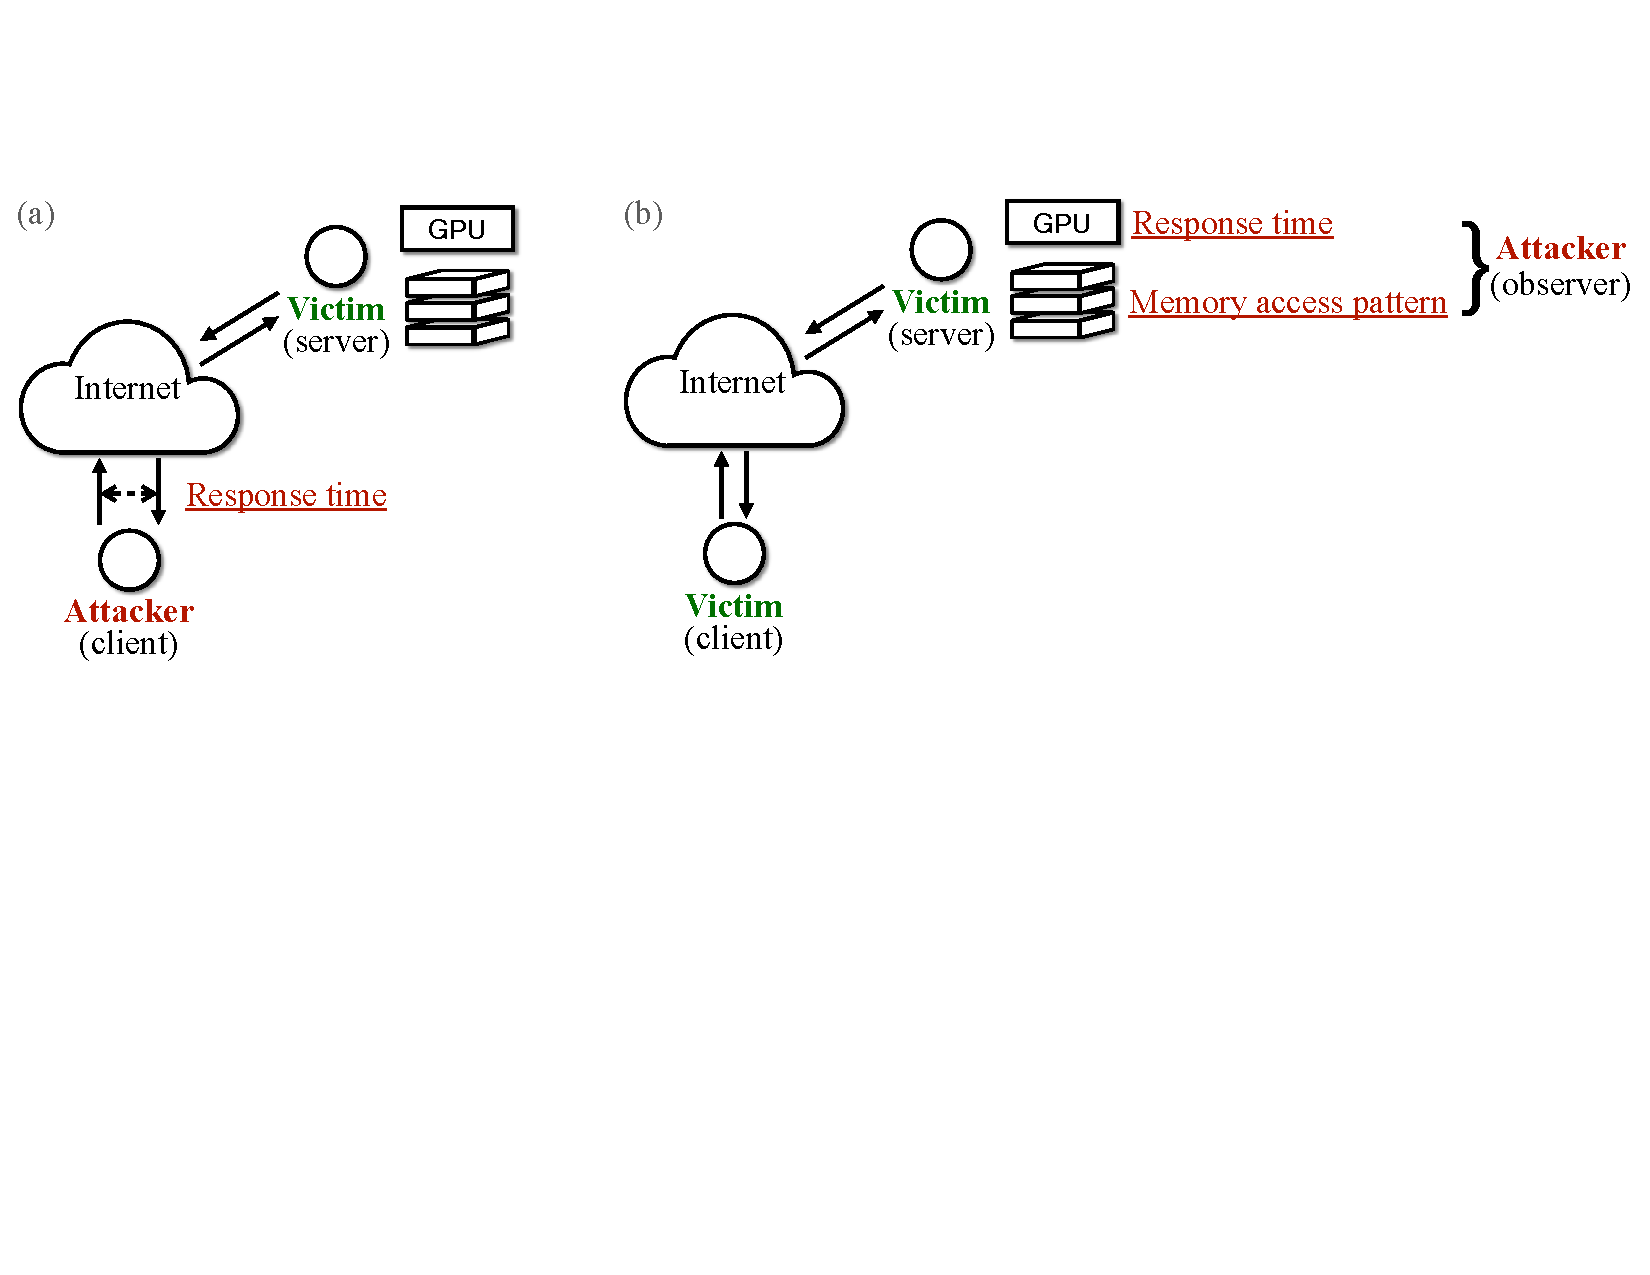
\includegraphics[clip,trim=0 10cm 0 2cm,width=0.72\pdfpagewidth]{figs/thrust1-fig.pdf}
    \caption{Attacker model considered in Thrust 1 \farzaneh{add quantitative?}}
    \label{fig:th1-attack}
\end{figure}

In order to mitigate these timing channel attacks through memory accesses, we propose a relational, resource-aware program logic capable of proving facts about the difference in execution time between two runs of a program.
%
This logic is sufficient to guarantee that execution time is independent of secret input (a security property known as {\em noninterference}), but is quite heavyweight and likely to require some programmer annotation.
%
We additionally develop an IFC type system which tracks the security level of data as it moves through a program and disallows memory accesses that could leak secure information; the type system is necessarily more conservative than the program logic, but much easier to work with in practice and uses the program logic to gain precision at strategic points.

\paragraph{Thrust 2. Active attacks}
In the attacks we consider in Thrust 2, the attacker has their own process in the cloud (as a client) which coexists with the victim process.
%
The victim and attacker both use the GPU server on the cloud and, through leaks caused by reuse of the registers and memory locations between processes, can gain access to the contents of the victim process's address space.
%
See Figure~\ref{fig:th2-attack}

\begin{figure}[h]
    \centering
    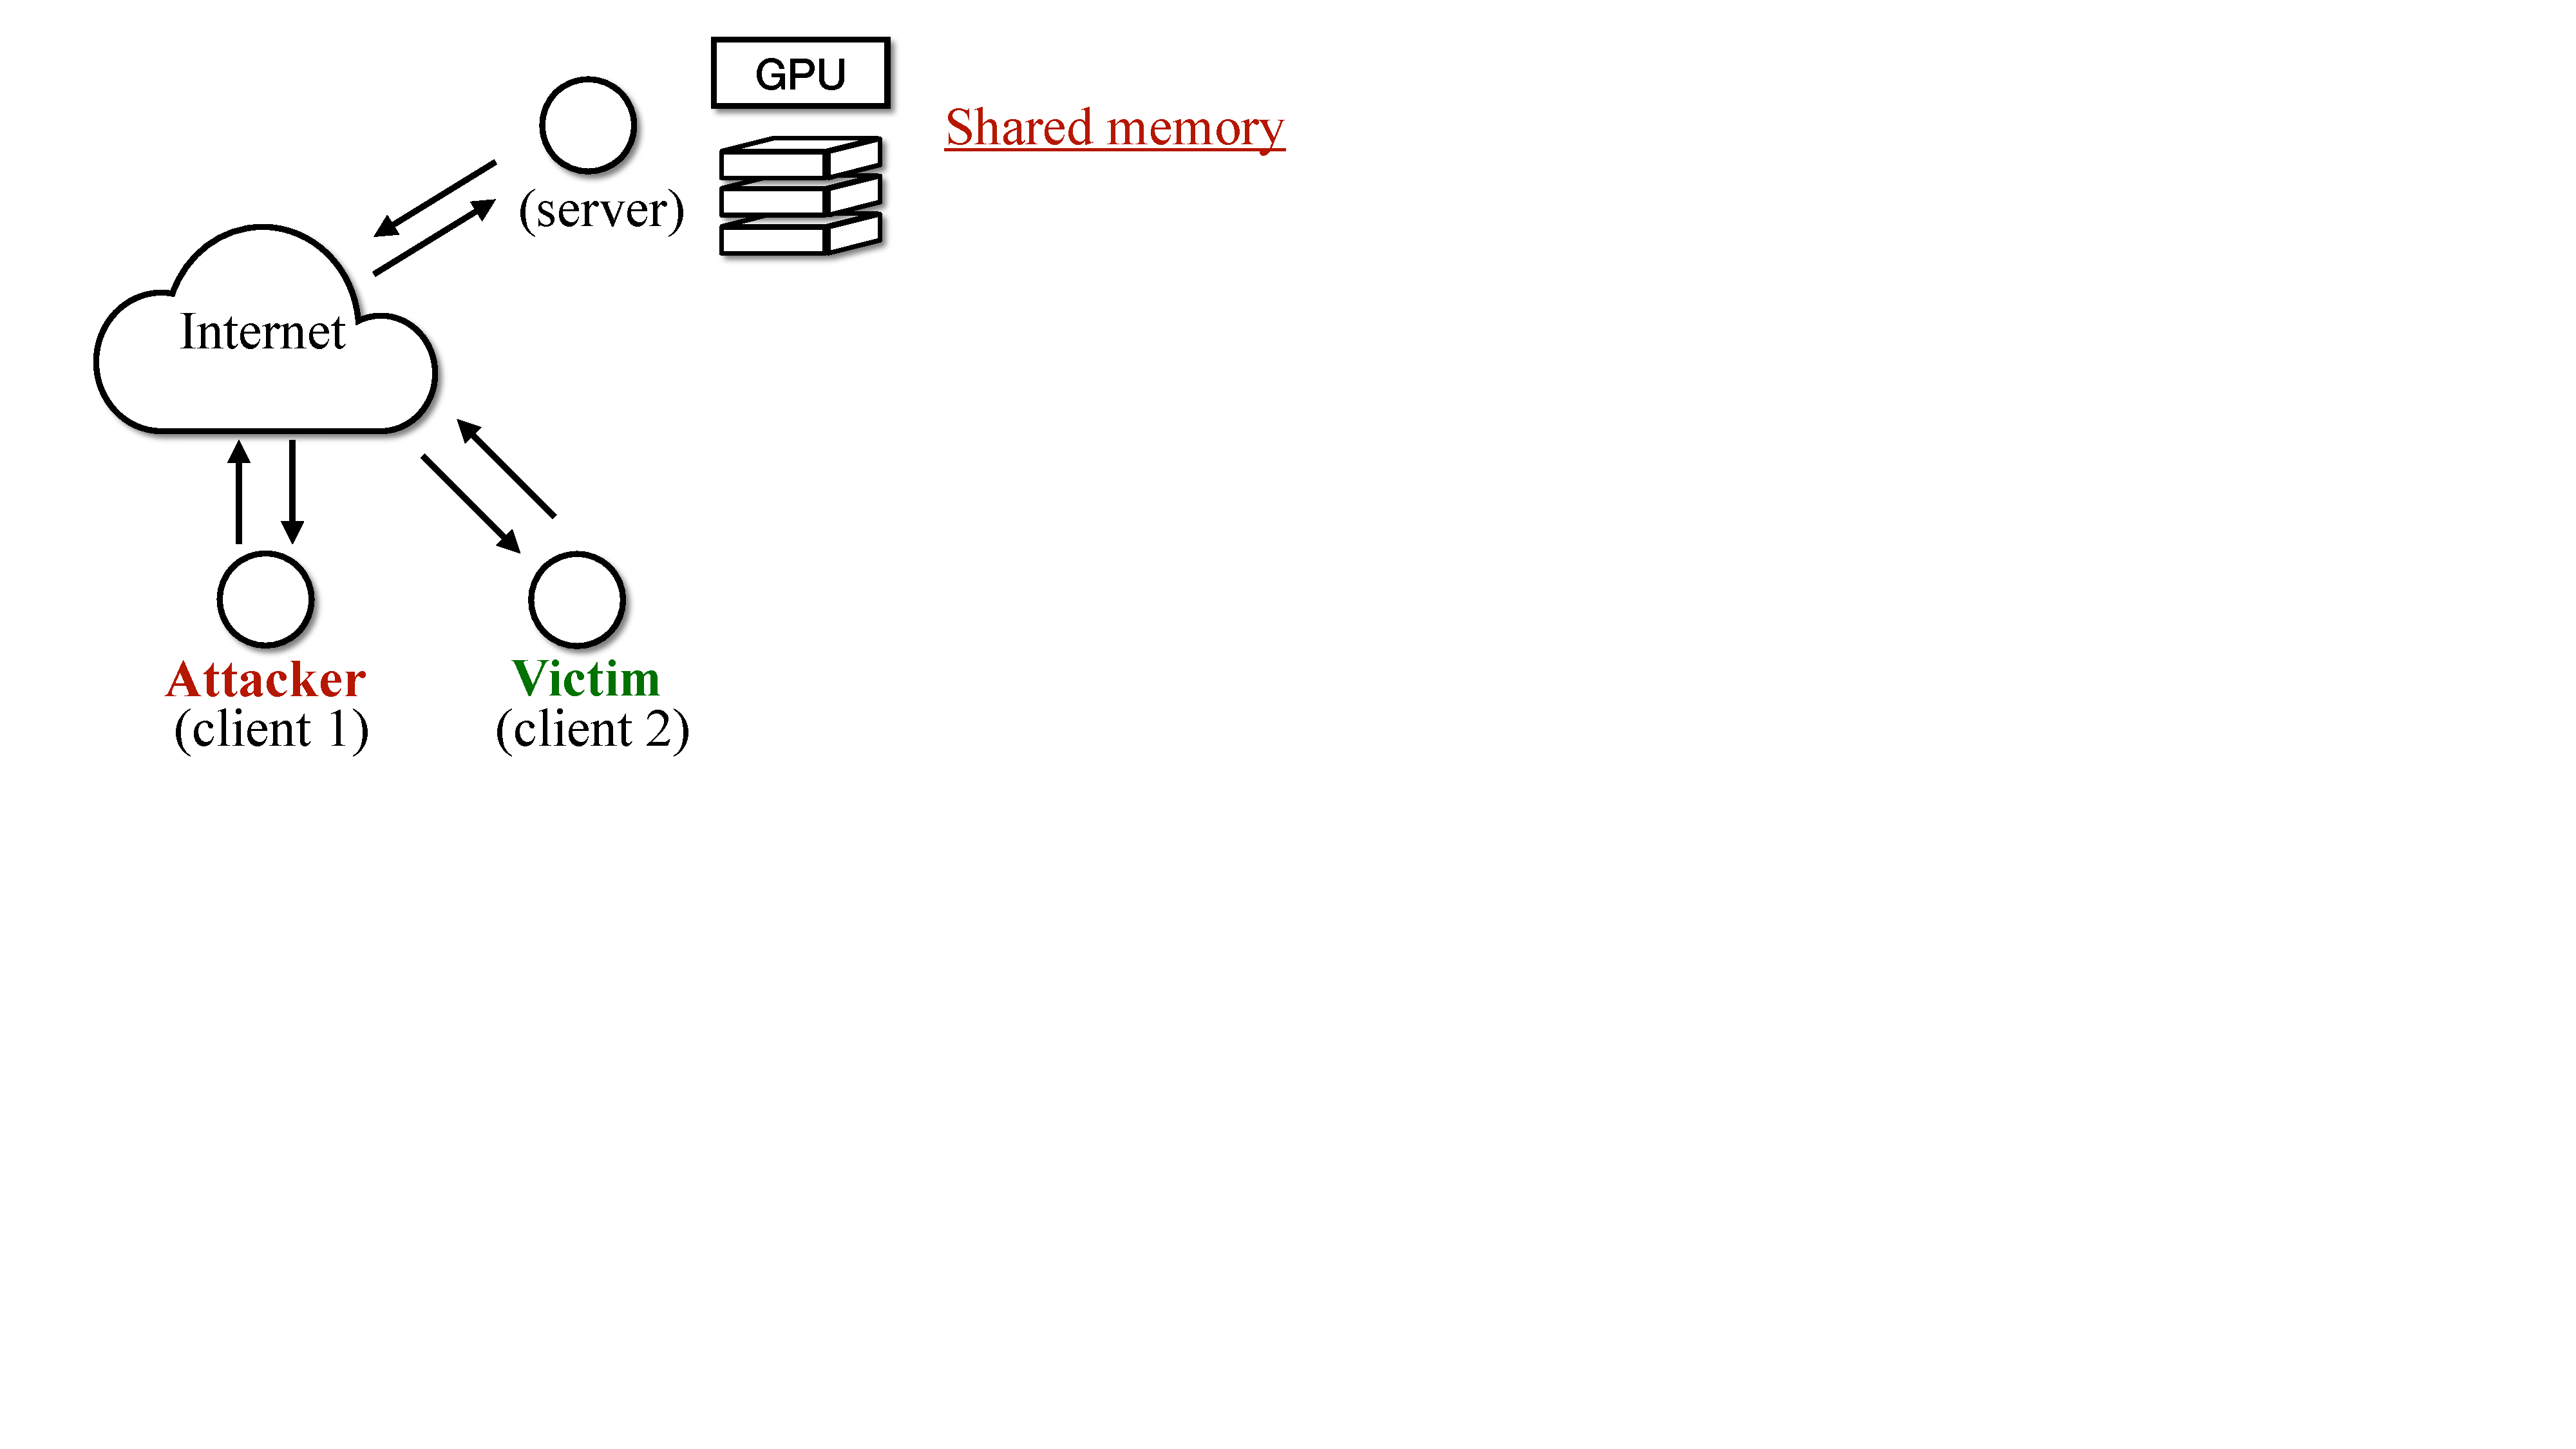
\includegraphics[clip,trim=0 17cm 10cm 0cm,width=0.72\pdfpagewidth]{figs/thrust2-fig.pdf}
    \caption{Attacker model considered in Thrust 2 \farzaneh{add more}}
    \label{fig:th2-attack}
\end{figure}

\stefan{Talk about what we do.}


\paragraph{Thrust 3. Case study}
In Thrust 3, we implement two case studies (AES encryption and a Large Language Model application) which have been previously shown to be vulnerable to the attacks described in the first two thrusts.
%
We will show that these vulnerabilities are detected by the type system and program logic of Thrust 1, both in theory and using the implementations of the type system and program logic that we will build as part of the thrust.
%
We will then demonstrate the Thrust 2 vulnerabilities by implementing an attacker process that can run alongside the case study applications and take advantage of information leaks.
%
Finally, we plan to create patched versions of the two case studies and demonstrate that the security vulnerabilities have been mitigated.


\subsection{PI Qualifications}

PIs Derakhshan and Muller will work closely together to complete the objectives
of the proposal.
%
Both PIs are in the Programming Languages group at Illinois Tech, and have been
working closely together since PI Derakhshan joined the faculty, including
coadvising a number of students, one of whom has begun preliminary studies
on the proposed work.
%
PI Derakhshan is an expert on language-based security \stefan{expand}.
%
PI Muller is an expert in static resource analysis, and has previously
conducted a successful NSF-funded study on static resource analysis for CUDA.
%
As part of this work, PI Muller and his students and collaborators
developed an operational semantics for CUDA as well as a resource-aware
program logic (and an OCaml implementation of it) for predicting the impact
on execution time of CUDA performance characteristics such as the ones
that lead to the described vulnerabilities~\cite{MullerHo21}.
%
We plan to use this logic and its implementation as a starting point for
our work.

\subsection{Broader Impacts}

With the rise of machine learning and large language models, and the recognition that the parallel performance of GPUs is necessary to achieve the required scaling, GPU computing has become a multi-trillion-dollar industry.
%
However, a number of recent high-profile leaks have made consumers understandably wary of the use of their private data.
%
Understanding the security risks of GPU computing and how to mitigate them is of paramount importance to the continued success of this burgeoning area.
%
In addition to the clear benefits to society, this project will provide numerous opportunities for student research, including undergraduate research, at Illinois Tech, an R2 research university with a demographically and economically diverse student body.
%
We discuss the broader impacts of the proposal in more detail in Section~\ref{sec:impacts}.


\section{Background and Related Work}
\label{sec:background}
In this section, we discuss the GPU execution model, focusing on characteristics that lead to the vulnerabilities we propose to study.
%
We also discuss related work on formal models of CUDA and security for GPU programs.
% Extras: 

% One prominent task is inference of neural networks, which process vast amounts of personal data, such as audio, text or images.


% Typically, AI is used for
% the evaluation of large datasets, from processing medical
% data to automated evaluation of surveilance feeds. Today,
% AI suitable for everyday use has arrived at the hands
% of the end-user in the form of Large Language Models
% (LLMs) [

% Hence, a lot of business cases for the utilization of
% LLMs have emerged, ranging from automatically handling
% customer service requests to tasks such as text content
% generation

% offer GPU-asa-
% Service (GaaS), where users can rent GPUs on demand
% and pay via a usage model. Customers can enjoy a high
% degree of flexibility, renting GPU computational power
% on demand.

% Allocating a complete GPU
% to a single container or virtual machine (VM) can be
% considered a waste of resources if either only a fraction
% or only a limited time of processing power is needed. The
% ability to share GPUs gives the provider a cost-effective
% measure to adapt to varying workloads. As industrial
% examples, Google’s Kubernetis Engine allows to share
% a GPU between up to 48 tenants, while Microsoft build
% GPU Paravirtualization into the Hyper-V Hypervisor, allowing
% VMs to share a single GPU



\paragraph{Parallelism and Memory Behavior in GPU.}
Threads on a GPU (of which there may be thousands) are organized into groups
called {\em warps}.
%
We will use the identifier \texttt{warpsize} to refer to the number of threads
per warp, which is~32 on all implementations of which we're aware.
%
Warps are organized into {\em blocks}, and blocks are grouped into {\em grids}. The dimensions of blocks and grids are specified when the kernel is launched.
%
Each thread has a unique thread ID within its block, and each block has a unique block ID within the grid, enabling scalable parallel execution.
%
GPUs utilize Single Instruction, Multiple Thread (SIMT) execution to run the same arithmetic or logical instruction on many threads simultaneously.
%
All threads within a warp must execute the same instruction, although some threads may remain inactive during execution.

Registers are the fastest type of memory in CUDA and are private to each thread, allowing quick access to frequently used variables. 
%
{\em Shared memory} is a smaller, but faster, memory space accessible to all threads within a block, enabling efficient data sharing and coordination. 
%
{\em Global memory} is the largest memory space, accessible by all threads across different blocks, but it is much slower compared to registers and shared memory.

\paragraph{Shared Memory and Bank Conflicts.}
Shared memory, like other types of memory, must be loaded into registers before operations can be performed on it.
%
Because all active threads within a warp perform the same instruction simultaneously, they will all perform simultaneous requests to shared memory, but potentially from different addresses.
%
Memory locations in shared memory are assigned to~32 ``banks'' in hardware.
%
Each bank can retrieve or store to only one address at a time.
%
All 32 banks can simultaneously deliver words to all 32 threads of a warp quickly, provided that each bank is requested for only one word.
%
When multiple words are requested from the same bank by different threads within a warp, a {\em bank conflict} occurs, causing the bank to access the words sequentially.
%
In the worst case, all 32 threads would read from different addresses within the same bank, and 32 sequential memory accesses would be performed.
%If all threads of a warp access the same word from shared memory, a broadcast operation takes place, where the memory is read once and the value is distributed to all threads. 
%
%This operation is as fast as conflict-free access to every bank.

\paragraph{Global Memory and L1/L2 Cache.}
As with shared memory, when an access to global memory occurs, all active
threads within a warp perform an access to global memory, but potentially on
different addresses.
%
The GPU attempts to coalesce these accesses into actual memory transactions
or {\em sectors},
each of which accesses a fixed number of bytes (e.g., 32 or 128) at a time,
consisting of multiple words.
%
If memory accesses within a warp display a high degree of spacial locality,
the access may need fewer sectors, and therefore a smaller latency, to serve
the requests.
%
In the worst case, if threads within the warp all access very distant
addresses (the memory access is {\em uncoalesced}), many more sectors might
need to be accessed.

The property of global memory described above both compounds and interacts with
the usual effects of caching on memory access latency.
%
GPUs have L1 and L2 caches which behave in a similar way to those of CPUs.
%
As in ordinary CPU programs, memory accesses with a high degree of locality increase the probability of cache hits and therefore better performance.
%
In addition, accesses to the L1 and L2 caches are coalesced in the same way described above, but the size of a sector may differ between the L1 and L2 cache.

%\farzaneh{From NVIDIA:
%Memory accesses that are cached in both L1 and L2 (cached loads using the generic data path) are serviced with 128-byte memory transactions whereas memory accesses that are cached in L2 only (uncached loads
%using the generic data path) are serviced with 32-byte memory transactions. Caching in L2 only can therefore reduce over-fetch, for example, in the case of scattered memory accesses.}




\paragraph{Related work on Modeling Execution Cost of CUDA.}
In prior NSF-supported work~\cite{MullerHo21}, PI Muller and his collaborator Jan Hoffmann developed MiniCUDA, a core calculus for CUDA with a formal dynamic semantics modelling the execution behavior of CUDA kernels on GPUs, including its cost of execution, taking into account factors such as bank conflicts and coalescing of global memory accesses.
%
The work also included a quantitative program logic for predicting the execution cost of a MiniCUDA kernel in terms of a provided {\em resource metric}, which can count any desired combination of bank conflicts, global memory transactions, and other features.
%
We plan to use MiniCUDA as the basis of our language model, and the semantics and quantitative program logic as a starting point for proving the soundness of our type system: our type system should guarantee that two runs of the kernel on states that differ only in high-security memory locations shouldn't differ in their observable execution behavior, including cost.
%
Muller and Hoffmann's implementation of the quantitative program logic, called RaCUDA, can also serve as a starting point for our implementation of the type system.

\paragraph{Related works on GPU security.}
\stefan{TODO Farzaneh: complete}
(With a microbenchmark they measured the
time for a sequence of memory accesses of each thread in a block.)
%
The attack strategy commonly deployed in CPU-based. timing attack methods consist of one block of ciphertext, and profiling the associated time to process that
block. However, on a GPU it would be the encryption workload would contain multiblock messages, and on each data sample, the GPU
timing attackwould produce many blocks of ciphertext.
The key difference is that the GPU scenario will only
collect a single timing value for the multiple blocks.
Although many successful attack methods have been
demonstrated on CPU platforms, these methods cannot be directly applied to the GPU platform due to a
lack of accurate timing information and nondeterminism in thread scheduling.

\paragraph{Symbolic GPU security.}




\section{Motivating Examples}
\label{sec:motivating}
In this section, we discuss two motivating examples drawn from recently
published timing attacks on GPU code.
%
We will refer to these examples throughout the proposal and, in Thrust 3,
propose to reproduce the attacks and show that our proposed work mitigates
them.

\subsection{AES Encryption}
Advanced Encryption Standard (AES) is one of the most popular encryption algorithms.
%
Given a cipher key, the AES algorithm applies iterative rounds of transformations  to encrypt a confidential input (plaintext) such as passwords and private messages into the ciphertext.
%
Each round constructs a new {\em round key}, and all round keys are considered
to be high-security as any one is sufficient to reconstruct the original
secret.
%
In each round, a transformation is applied to 16-byte blocks of the round key.
%
In order to speed up encryption, many implementations of AES implement the
transformations partially using a lookuptable: each byte of the block is
looked up in the table to obtain a transformed byte, and then an additional
operation is performed on the transformed bytes within the block.
%
Because blocks can be encrypted independently and the same lookup table is used
for all of the transformations in a round, it is logical to parallelize
encryption by having each thread transform a block, and to store the lookup
table in shared memory.

Because the table is stored in shared memory and is indexed using bytes of the
round key, the number of bank conflicts can leak information about the key.
%
Jiang et al.~\cite{AESattack} present such an attack on a table-based
implementation of AES, and show that they are able to reconstruct the
last-round key solely by observing the encryption time.

\subsection{merge}
We also consider the scenario in which both the victim and attacker are clients of a shared GPU (see Figure~\ref{fig:th2-attack}). 
%
Several prior sudies~\cite{lee} showed that if the attacker's application runs on the same GPU as the victim's, it can potentially access private information left on the GPU memory by the victim's application.
%
% This potential leak occurs both in a sequential time-sharing setting and in a concurrent setting, e.g., enabled by NVIDIA Multi-Process Service (MPS).
%
Multiple GPU processes are executed in an interleaved fashion, with each process having exclusive access to GPU resources for a defined duration. The kernels of these processes are scheduled to run one after the other.
%
% In the concurrent setting, multiple GPU processes can share GPU resources simultaneously, enabling multiple kernels to run at the same time.
%
% In both cases, a 
A lack of proper memory isolation may lead to an overlap between the memory locations that the attacker can access through normal operations—without any special privileges—and those used by the victim.
%
%
% If the attacker's application runs concurrently with the victim's, it can potentially access private information that is left on the GPU memory by the victim's application.
%
% if the memory locations allocated to the attacker overlap with those used by the victim.
%
% To achieve this, the attacker only needs to access the GPU memory through regular allocation, deallocation, and read/write operations without requiring any special privileges.
%
The details of the attack vary depending on where in the memory the victim's information is located, e.g., in the shared or global memory, and whether the GPU server is concurrent or sequential.
%

Figure~\ref{fig:th2-mot}(a), for example, demonstrates an attack on a server with private information stored in shared memory.
%
The victim in this scenario is an AES application.
% 
GPU computing models discourage long-running GPU kernels. 
%
Thereby, the AES application uses several kernels, instead of a long-running one, repeatedly and processes the intermediate results. 
%
To increase efficieny, the application keeps its frequently accessed data, e.g., the encryption key, in shared memory, even after a single kernel terminates.
%
This means that if an attacker's kernel is scheduled to run between two kernels of the victim, it can compromise the security of the plaintext. 
%
The attacker can compromise the security by either reading the data left in shared memory, eventually relaying it back to the attacker's CPU (through either a direct or indirect leak), or by overwriting the data, altering the key.
%
In both cases, the attacker knows the key and can infer the plaintext by observing the public cyphertext. 
%
In the literature, this attack is often called the End of Kernel (EOK) attack.


Figure~\ref{fig:th2-mot}(b) demonstrates a similar attack for a  server, but this time with the private information stored in global memory.
%
A segment of global memory is allocated to each CUDA context,  and an interleaved attacker kernel cannot access it until the application has terminated and the memory is deallocated.
%
After the application terminates, it deallocates the memory,  which then becomes available for future allocations.
%
However, prior work~\cite{pietro2016TECS} have demonstrated that data can persist even after deallocation, allowing an attacker kernel that runs immediately after the application to access the memory segment with its prior data. 
%
As such, even if the programmer attempts to clear the memory before exiting, this access can still result in information leakage. 
%
For example, in Figure~\ref{fig:th2-mot}(b), the attacker can access the plaintext stored in the global memory by the victim even after the deallocation of the global memory segment by the victim.
\subsection{Large Language Models}
\stefan{fill in}


\section{Thrust 1: A Secure Programming Model for CUDA}
%\subsection{Motivating Example: AES encryption algorithm.}

We briefly describe three main challenges in addressing timing attacks in GPU code.
%
Two of these challenges are specific to GPUs.
%
The third is a challenge for CPU security as well, but interacts with the
first two challenges and will need to be handled specially for GPU code.

\paragraph{Challenge 1: GPU-specific timing channels.}
The AES example in Section~\ref{sec:motivating} showed one new timing channel not addressed by prior work on CPUs: bank conflicts are a phenomenon specific to the GPU memory model.
%
While cache effects are a timing channel that exists in CPU code and also depends on locality of memory accesses \stefan{(cite? I assume someone has studied caching as a timing channel)}, bank conflicts behave differently and will need to
be handled differently.
%
For example, suppose~\texttt{h} is a high-security bit (i.e.,~\texttt{h} is known to be 0 or 1).
%
If array \lstinline{S} is stored in shared memory,
the access \lstinline{S[threadIdx.x * h]} has no bank conflicts regardless
of~\texttt{h} and therefore leaks no information through bank conflicts
(if \lstinline{S} contains secret data, it may, of course, leak this data
through other means).
%
Neither does the access \lstinline{S[threadIdx.x * 5 * h]}: because~5
and~32 are relatively prime, even if~\texttt{h = 1}, each thread targets a
different bank, although the locality is much worse.
%
However, the access \lstinline{S[threadIdx.x * 2 * h]}, which has better
locality than the previous code, will result in bank conflicts if~\texttt{h = 1}.

The SIMT execution model of GPUs can also lead to timing channels.
%
Consider the following code:

\begin{lstlisting}
if (h) {
  h = 1;
} else {
  h = 2;
}
\end{lstlisting}

Recall that each thread has a separate copy of local variables, so that
each thread may have a different value for~\texttt{h}.
%
The code results in no insecure information flows through data: only
high-security variables are written.
%
If this code is executing on a CPU using reasonably traditional cost models,
there are also no obvious timing channels: one branch will be taken, but
both should take the same amount of time.
%
However, because all threads of a warp must execute the same instruction at the same time, when a warp evaluates the conditional, if~\texttt{h} is true in some threads and false in others, the GPU must disable the threads where~\texttt{h} is false, run the ``then'' branch, and then swap what threads are active to execute the ``else'' branch.
%
The two branches run sequentially on different sets of threads.
%
This is referred to as a {\em warp divergence}.
%
If~\texttt{h} has the same value on all threads in the warp, however, only
one branch is executed.
%
This means that, when run on a GPU, the above code has a timing leak: by
observing the time taken to execute the code, we can determine whether or not
all threads in the warp have the same value for~\texttt{h}.

\paragraph{Challenge 2: Leaks through the thread mask.}
An additional difficulty in reasoning about GPU code, which is not present in CPU code, is that the security of a code snippet can depend on the current {\em mask}, that is, what threads in a warp are active (which may be a subset of the threads in the warp if there has been a warp divergence).
%
For example, consider the following program in which~\lstinline{h} is a high-security local variable,~\lstinline{S} is an array stored in shared memory, and~\lstinline{threadIdx} is the integer thread identifier of each thread.

\begin{lstlisting}
if (h) {
  S[2 * threadIdx] = 0;
} else {
  S[2 * threadIdx] = 0;
}
\end{lstlisting}

Naively, it would appear that, although this program conditions on the high-security variable~\lstinline{h}, doing so can't leak information because the code in both branches is identical and the shared memory access uses only low-security indices (\lstinline{threadIdx} is considered low-security).
%
However, the program does indeed leak information.
%
Consider an execution in which threads 0--15 take the ``then'' branch and threads 16--31 take the ``else'' branch.
%
In this case, neither branch has a bank conflict, and nor does the program as a whole because the two branches are executed in sequence.
%
On the other hand, consider an execution in which even-number threads take the ``then'' branch and odd-number threads take the ``else'' branch.
%
In this case, both branches have a bank conflict.
%
The leak here is due to the fact that {\em which threads are active} during each branch impacts cost behavior, and this in turn is determined by high-secrecy information.
%

Because GPU programs generally have thousands of threads, reasoning about the local state of individual threads quickly becomes intractable.
%
Muller and Hoffmann~\cite{MullerHo21} observe that a useful middle ground is to instead track which variables are {\em uniform} across all threads and reason precisely only about the local state of these variables.
%
From a cost perspective, this is sufficient in many real-world GPU programs because variables, such as loop indices, that impact cost are generally uniform.
%
We hypothesize that this approximation is useful in a security context as well.
%
For example, in determining that the above program has an information leak, it suffices to know {\em whether}~\lstinline{h} is uniform, because the leak stems from the fact that it may be divergent (i.e., not uniform).


\paragraph{Challenge 3: Quantitative leak analysis.}
Avoiding any possibility of information leaks is too restrictive and also not realistic: in the AES example, it is difficult to imagine any table-based implementation that would not suffer from possible timing attacks; even if preventing these attempts is possible, it would be at the cost of a very slow implementation.
%
However, small differences in the number of bank conflicts may not even be detectable by the attacker given the nondeterministic environment and experimental noise.
%
This suggests there may be some middle ground where the differences in bank conflicts between runs are mitigated to the point where extracting a key based on differences in timing is intractable but the implementation is still reasonable.
%
Moreover, even if the attacker observes some information it is ok if we leak some sort of information (another reason why LLM is a betetr example).
%
If we are too restrictive and avoid every form of leakage, then we cannot train LLM at all. \stefan{This sounds more related to declassification, which we don't address; maybe I'm misreading it.}
%
What we want however, is to ensure that the information that attackers' observations do not increase their chances of guessing private information beyond some acceptable amount.
% The key is fixed. Test it using a given plaintext to find the key.
% Accessing shared memory depends on the key.



%

% AES: shared memory accesses are dependent on the key. 
% %






% As the constant cache stores data
% from constant memory that can be shared by threads
% in a warp, for AES encryption we use this space to store
% round keys.


\subsection{Proposed work}
\subsubsection{Task 1.a. Information Flow Control Type System for GPU Timing Attacks}

Our goal in this task is to statically ensure information security of GPU kernels, and in particular their invulnerability to timing attacks.
%
Our security condition in this task will be {\em cost-sensitive noninterference} \stefan{Is there an existing term for this?} for individual GPU kernels.
%
We define this condition as follows: assign a {\em security level} to every local variable and array in a kernel indicating the secrecy of its contents---for example purposes, we will consider security levels High (high secrecy) and $\bot$ or Low (not secret), but the techniques apply to general lattices of security levels.
%
Consider two executions of a program, starting with memories that agree on variables of security level less than~$\seclevel$ but may differ on higher-security variables.
%
We call such starting points {\em low-equivalent} states.
%
Cost-sensitive noninterference at a security level~$\seclevel$ requires that two executions of a program, starting with low-equivalent states, are indistinguishable in their input-output behavior, effect on low-security memory locations, and observable cost behavior.
%
For most of the examples in this proposal, ``observable cost behavior'' means number of bank conflicts, but in our proposed work, we plan for this to also include number of memory transactions and other performance characteristics closely tied to program data.

In this task, we ensure cost-sensitive noninterference through two main mechanisms.
%
First, we develop a resource-aware Relational Hoare Logic for quantitatively bounding the difference in execution cost between two evaluation of a statement or expression (e.g., that differ only on high-security memory locatins).
%
This logic is sufficient to ensure noninterference and is quite powerful in specifying fine-grained policies.
%
However, it suffers from the same drawbacks as program logics in general: they are often not decidable and require significant human interaction and/or advanced heuristics to prove complex properties such as noninterference.
%
To complement these drawbacks, we will develop an information flow control (IFC) type system that tracks security levels of expressions and statements throughout the program and disallows operations that might violate cost-sensitive noninterference.
%
At key points, for example at a conditional where the condition depends on high-security information, the type system must ensure that the execution costs (e.g., bank conflicts, memory accesses) of the two branches are identical.
%
It does this by ``calling out'' to the Relational Hoare Logic.
%
Uses of the more general logic are therefore localized, reducing the burden on programmers and analysis tools.

We show the soundness of our approach in two steps.
%
First, we show that the Relational Hoare Logic is sound with respect to an operational model of GPU execution.
%
As the model, we plan to use the operational semantics of MiniCUDA~\cite{MullerHo21}, which also track abstract execution cost including bank conflicts and memory accesses.
%
Second, we will show the type system sound with respect to the Relational Hoare Logic, i.e., a well-typed program is related to itself in that any two executions with low-equivalent starting states have the same cost and observable behavior.

\farzaneh{Put more here based on Amal and Jan's RHL.}

A key difficulty in analyzing GPU programs, as opposed to CPU programs, is that each thread maintains a separate copy of local variables.
%
This fact can be used to leak information in non-obvious ways.
%
For example, consider the following program in which~\lstinline{h} is a high-security local variable,~\lstinline{S} is an array stored in shared memory, and~\lstinline{threadIdx} is the integer thread identifier of each thread.

\begin{lstlisting}
if (h) {
  S[2 * threadIdx] = 0;
} else {
  S[2 * threadIdx] = 0;
}
\end{lstlisting}

Naively, it would appear that, although this program conditions on the high-security variable~\lstinline{h}, doing so can't leak information because the code in both branches is identical and the shared memory access uses only low-security indices (\lstinline{threadIdx} is considered low-security).
%
However, the program does indeed leak information.
%
Consider an execution in which threads $0--15$ take the ``then'' branch and threads $16--31$ take the ``else'' branch.
%
In this case, neither branch has a bank conflict, and nor does the program as a whole because the two branches are executed in sequence.
%
On the other hand, consider an execution in which even-number threads take the ``then'' branch and odd-number threads take the ``else'' branch.
%
In this case, both branches have a bank conflict.
%
The leak here is due to the fact that {\em which threads are active} during each branch impacts cost behavior, and this in turn is determined by high-secrecy information.
%

Because GPU programs generally have thousands of threads, reasoning about the local state of individual threads quickly becomes intractable.
%
Muller and Hoffmann~\cite{MullerHo21} observe that a useful middle ground is to instead track which variables are {\em uniform} across all threads and reason precisely only about the local state of these variables.
%
From a cost perspective, this is sufficient in many real-world GPU programs because variables, such as loop indices, that impact cost are generally uniform.
%
We hypothesize that this approximation is useful in a security context as well.
%
For example, in determining that the above program has an information leak, it suffices to know {\em whether}~\lstinline{h} is uniform, because the leak stems from the fact that it may be divergent (i.e., not uniform).
\stefan{Move this example to an earlier section?}

\paragraph{Resource aware - Relational Hoare Logic.}
The judgment for our resource-aware Relational Hoare Logic will be of the form 
%
\[\{\Phi; Q; X\} p_1 \sim p_2 \{\Phi'; Q'; X'\}\]
%
where $p_1$ and $p_2$ are programs the we want to relate (they may be the same program, in which case we relate two executions).%
The logical preconditon $\Phi$  describes the relation between the two states before running programs $p_1$ and $p_2$. 
%
The {\em potential function} $Q$ maps program states to rational numbers.
%
Such a function is familiar from the potential or ``physicist's'' method of amortized analysis, where certain operations accrue potential (analogous to potential energy in physics) in the program state that can then be used to amortize the cost of periodic expensive operations.
%
Our Relational Hoare Logic utilizes a non-standard interpretation of the potential function: the potential actually pays for the {\em difference} between the two execution costs.
%
If the two programs evaluate in lockstep, performing identical memory transactions and other observable operations, no cost is accrued.
%
As discussed earlier \stefan{keep track of where}, we only want to reason about the values of variables that are known to be uniform across all threads; this means that only the states of such variables are included in~$Q$.
%
We keep track of these variables using the third component of the precondition, $X$, which is itself a pair $(X_1, X_2)$ of sets of variables.
%
Sets~$X_1$ and~$X_2$ contain the variables known to be uniform before executing~$p_1$ and~$p_2$, respectively.
%
Moving to the postcondition, $\Phi'$ describes the relation between the two states after running programs $p_1$ and $p_2$; $Q'$ is a potential function for the remaining potential after paying for any differences in cost between $p_1$ and $p_2$, and $X'$ contains the sets of uniform variables in the two executions after executing the two statements.

We will need two forms of rules, {\em synchronous} and {\em unscynchronous}.
%
The synchronous rules relate two executions of the same form of statement;
for example, here is the rule that relates two assignments to shared memory. 
\[
\infer[]{ \Phi[e_1/S_1[o_1]][e_2/S_2[o_2]] \Rightarrow \mathtt{diff\_conflicts}(o_1,o_2) \le n\\  \Phi \vdash e_1 \sim e_2 : m}{\{\Phi; Q+n+m; X\} S_1[o_1] \leftarrow e_1 \sim S_2[o_2] \leftarrow e_2 \{\Phi; Q; X\}  }
\]
The premise~$\Phi \Rightarrow \mathtt{diff\_conflicts}(o_1,o_2) \le n$ indicates that, under the logical conditions in~$\Phi$, it is possible to reason that the difference in the number of bank conflicts between the two indices~$o_1$ and~$o_2$ is less than~$n$.
%
For example, if~$\Phi$ guarantees that~$o_1 = o_2$, then we can conclude~$ \mathtt{diff\_conflicts}(o_1,o_2) = 0$.
%
The auxiliary judgment~$\Phi \vdash e_1 \sim e_2 : m$ states that the difference in the number of bank conflicts triggered by~$e_1$ and~$e_2$ is bounded by~$m$.
%
The rules for this judgment mainly relate shared memory accesses in subexpressions of~$e_1$ and~$e_2$ using~$\mathit{diff\_conflicts}$.
%
In the conclusion of the rule, the main change between the pre- and post-conditions is a cost of~$n + m$ to pay for the maximum possible difference in bank conflicts between the two programs.
%
We also include the information about the assignment in~$\Phi$ by substituting the assigned expressions for the target locations in the precondition, as is standard in Hoare Logic.

The asynchronous rules relate two different forms of statements, and are necessary for, e.g., relating the two branches of a conditional to guarantee that the choice of branch can't leak information through timing channels.

We prove soundness of the Relational Hoare Logic by comparing it to the cost-annotated operational model of CUDA execution developed by Muller and Hoffmann~\cite{MullerHo21}.
%
The operational semantics judgment is~$\sigma; p \Downarrow^{\mathcal{T}}_m \sigma'; n$.
%
In this judgment,~$\sigma$ and~$\sigma'$ are {\em states}, i.e., the values of local variables and arrays, before and after execution.
%
We write~$\Phi \vdash (\sigma_1, \sigma_2)$ to mean that a pair of states satisfies a condition~$\Phi$ in that the states and the relation between them satisfy all of the logical conditions specified in~$\Phi$.
%
The program~$p$ executes with the set~$\mathcal{T}$ of active threads (this may be a subset of all threads if warps have diverged).
%
The judgment also indicates the cost~$n$ of execution in units specified by a {\em resource metric}~$m$, which assigns costs to program operations and conditions---in our example, we would use a resource metric that assigns a cost of~$m$ to an~$m$-way bank conflict and a cost of zero to all other operations.
%
The soundness theorem for the logic states that, if we execute~$p_1$ and~$p_2$ starting with states that satisfy~$\Phi$, the difference in potential predicted by the logic overestimates the actual cost difference between the two executions:

\begin{theorem}[Soundness of Relational Hoare Logic]\label{thm:logic-sound}
If~$\Phi \vdash (\sigma_1, \sigma_2)$ and
$\{\Phi, Q, \{\}\} p_1 \sim p_2 \{\Phi', Q', X'\}$
and $\sigma_1; p_1 \Downarrow^{\mathcal{T}}_m \sigma_1'; n_1$
and $\sigma_2; p_2 \Downarrow^{\mathcal{T}}_m \sigma_2'; n_2$
then $|n_1 - n_2| \leq Q(\sigma_1, \sigma_2) - Q'(\sigma'_1, \sigma_2')$.
\end{theorem}


\paragraph{IFC type system.}
The Relational Hoare Logic described above is sufficient to guarantee noninterferece.
%
We can guarantee that a program~$p$ satisfies noninterference by requiring the
provability of the triple
\[\{\Phi; 0; \{\}\} p \sim p \{\Phi'; 0; \{\}\}\]
where~$\Phi$ is a condition that requires only that the two initial states be low-equivalent.
%
The soundness theorem guarantees that if the triple is provable, then the two executions of~$p$ do not differ in their resource usage.
%
However, proving such a triple may be quite cumbersome and there is no guarantee that doing so would be possible without substantial human effort.
%
We therefore develop a more conservative, but simpler and decidable, type system.

Information flow control (IFC) type systems typically extend conventional type systems by tracking the security level of variables in addition to their data types.
%
In doing so, the type system can, for example, restrict assignments that would
cause high-security information to flow to a low-security variable.
%
In CUDA, we need to track not just the security level of variables and
expressions but also
whether or not they are uniform across threads, because conditioning on
non-uniform expressions can cause leaks, as shown in \stefan{Example}.
%
Types in our type system are~$\tau_{\lpair{\seclevel}{\divergence}}$
where~$\tau$ is a standard data type such as $\mathsf{int}$, and
$\seclevel$ is a security level (we will use~$\bot$ for low-security and~$\top$
for high security; in general these can be values from an arbitrary security
lattice).
%
The component~$\divergence$ is either~$\dunif$ meaning ``uniform across
threads'' or~$\ddiv$ meaning ``possibly divergent (non-uniform) across threads.''
%
We can also treat pairs~$\lpair{\seclevel}{\divergence}$ as elements~$P$ of a
single lattice formed by taking the Cartesian product of the security
lattice with $\{\ddiv, \dunif\}$ and extending the join and ordering operators
in the natural way (uniform values may flow to non-uniform variables but not
vice versa).

Our typing judgment for CUDA statements~$s$ is
$\Sigma, \pc \vdash s$,
where~$\Sigma$ is a context providing the types of constants and variables,
and $\pc$ is the security level of the program counter, which makes the type
system flow-sensitive by indicating whether the control flow of the program
has been influenced by high-security information.


As an example, a general rule for assignments to shared memory might be:
\[
\infer[]
{ \Sigma(S) = \mathsf{arr}(\tau)_{\lpair{\seclevel_S}{\divergence_S}}\\
\Sigma, \pc \vdash o : \mathsf{int}_{\lpair{\bot}{\divergence_o}}\\
\Sigma, \pc \vdash e : \tau_{\lpair{\seclevel_e}{\divergence_e}}\\
(\pc \ljoin \seclevel_e) \secle \seclevel_S
}
{
\Sigma, \pc \vdash S[o] \leftarrow e
}
\]
The assignment is permitted as long as 1) the array index~$o$ is public
(since using a secret index could leak information through the number of
bank conflicts)
and 2) the security level of array~$S$ is at least as high as the
join of~$\pc$ and the security level of~$e$.
%
Clearly~$\seclevel_S$ must be higher than~$\seclevel_e$ as we are writing~$e$
into~$S$.
%
Using the level of the program counter prevents so-called {\em indirect flows}
such as this one, which also writes the value of the boolean~$b$ into~$S[0]$:
\begin{lstlisting}[language=C]
if (b) S[0] = 1;
else S[0] = 0;
\end{lstlisting}

Note that writing to shared memory when the program counter is impacted by
secret information is allowed; disallowing this would be safe, but unnecessarily
restrictive.
%
Instead, we prevent indirect leaks through bank conflicts with the rules
for \texttt{if}.

When conditioning on public information, it suffices to check that both
branches are well-typed:
\[
\infer[]
{\Sigma, \pc \vdash e : \mathsf{bool}_{\lpair{\bot}{\divergence_e}}\\
\Sigma, \pc \vdash s_1\\
\Sigma, \pc \vdash s_2
}
{\Sigma, \pc \vdash \mathsf{if}~e~\mathsf{then}~s_1~\mathsf{else}~s_2}
\]
Note that both branches are typed under~$\pc$ because conditioning on
public information does not increase the secrecy level of the program counter.

However, when conditioning on a secret, we need to ensure that no information
can be leaked through differences in the number of bank conflicts between the
two branches {\em or} through differences in the number of bank conflicts in
one branch that might result from differing sets of threads taking that
branch (see \stefan{Example}).
%
The type system lacks the precision to quantify the number of bank conflicts
and so, at this point, it is necessary to use the Quantitative Hoare Logic:
\[
\infer[]
{\Sigma, \pc \vdash e : \mathsf{bool}_{\lpair{\seclevel_e}{\divergence_e}}\\
\Sigma, (\pc \ljoin \seclevel_e) \vdash s_1\\
\Sigma, (\pc \ljoin \seclevel_e) \vdash s_2\\
\{\Phi; 0; \{\}\} s_1 \sim s_1 \{\Phi'; 0; \{\}\}\\
\{\Phi; 0; \{\}\} s_2 \sim s_2 \{\Phi'; 0; \{\}\}\\
\{\Phi; 0; \{\}\} s_1 \sim s_2 \{\Phi'; 0; \{\}\}\\
}
{\Sigma, \pc \vdash \mathsf{if}~e~\mathsf{then}~s_1~\mathsf{else}~s_2}
\]
We require that the number of bank conflicts in both branches is
unaffected by the set of active threads by relating each branch to itself,
and we require that the two branches have the same number of bank conflicts
under any differences in secret information by relating them to each other.

We prove soundness of the IFC type system by showing that well-typed programs
are related to themselves with empty starting potential.
Composing this result with Theorem~\ref{thm:logic-sound} ensures that
two runs
of a well-typed program with low-equivalent starting configurations do not
differ in the number of bank conflicts.

\begin{theorem}[Soundness of Type System]
If~$\Sigma, \bot \vdash p$
and~$\Phi$ is any condition requiring that the two starting configurations
be low-equivalent,
then $\{\Phi, 0, \{\}\} p_1 \sim p_2 \{\Phi', 0, \{\}\}$.
\end{theorem}



% Explain the type system.
% Relational Hoare Logic
% Logical relation

\subsubsection{Task 1.b.}
In Task 1.a. (\farzaneh{add the ref.}) we follow the classical approach of establishing noninterference to enforce security and ensure that no information is leaked to the attacker. This classical approach, however, is not always feasible or realistic. 
%
In a realistic setting, small leaks of information should be tolerated by the system as long as they are limited and do not significantly compromise the secrecy or identity of other parties.
% 
% Sometimes, certain information must be disclosed to a party with lower security clearance, but only in a way that does not significantly compromise the secrecy or identity of other parties. Sometimes, small leaks of information can be tolerated by the system as long as they are limited and do not increase the chance of guessing the secret by far. 
%
% An unreliable environment might induce noise in the observations of the attacker making the attacker unable to distinguish the difference between certain results, as long as the difference is is not ``too much''. 
% %
Even if the attacker observe different number of bank conflicts in two runs of the program, it may not be able to deduce ``too much'' information from it. 
%
% For example, the AES motivating example does not satisfy the noninterference property, since there is a flow of information from the high security information (plaintext) to low security information (cybertext).
% %
% However, this flow is designed in such a way that that 
% For example, because of the noise in the observations of the attacker, it cannot tell the difference between two execution times as long as the difference is ``not too much''. 
% %
% Or even if the attacker can observe the difference, it cannot deduce ``too much information'' from it. 
% %
The precise threshold for “too much'' varies depending on the specifics of the system. 
%
For example, in the motivating AES example, if the encryption key rotatation is set such that after every ten runs a new random key is generated, then leaking one bit of information in every run, cannot leak more than 10 bits of the ciphertext.
%
If we can quantify information leakage, we can compare it with the established threshold to ensure the system does not significantly compromise security.
%
In this task, we plan to maintain a realistic perspective on security by quantifying leaks via the timing side-channel.
\farzaneh{check the example above.}

We illustrate our approach using the example below.
%
The sample code works on a secret $h$ which stores a two bit value.
\begin{lstlisting}
    if (h=00) {
      S[2 * threadIdx] = 0;} 
    else {
      if (h=01) {
        S[threadIdx] = 0;}
      else {
        if (h=10) {
         S[2 * threadIdx] = 0;}
        else {
         S[threadIdx] = 0;}}}
\end{lstlisting}
% in Figure~\ref{fig:qtable}.
Based on the secret $h$, the program sends threads into four branches, in the first and third branches there are no bank conflicts, in the second and fourth branches there will be 16 bank conflicts.
%
The condition of the branch is not divergent, meaning that all threads will execute the same branch, but depending on the value of the secret the branch can be different.
%
We model the value of the secret $h$ as a random variable.
%
For now, let us assume that the probability distribution of the secret is uniform.
%
Meaning that each possible 2-bit secret value $s$ for $h$ has the same probability of $1/4$, i.e., $P(h=s)= 1/4$ for any $s\in S=\{00,01,10,11\}$.
%
The attacker knows this a priori probability, but cannot 
observe the exact secret stored in $h$; it is uncertain about the value of $h$.
%

Min-entropy provides a measure to quantify the amount of  uncertainty of the attacker (\cite{min-entropy}).
%
It is defined as 
$H_\infty(h)=-\log_2\max_s P(h=s)$,
and captures the probability that the attacker correctly guesses the secret in one try.
%
For example, before executing the program, the min-entropy is $H_\infty(h)=-\log_2\max_s P(h=s)= - \log_2 \max_s \{1/4,1/4,1/4,1/4\}= 2$.
%
We can interpret the min-entropy as the probability of the attacker guessing the correct secret is $1/2^{H_\infty(h)}$.
%
When the random variable has the uniform probability, one can rewrite a priori min-entropy as $H_\infty(h)=-\log_2\max_s P(h=s)=-\log_2 |S|$.
%
In this case, we can also interpret it as there are two bits that the attacker needs to know to fully guess the secret.
%

After executing the program, however, the attacker can observe the number of bank conflicts and learn information about the secret based on the number of observed bank conflicts.
%
If the attacker observes zero bank conflicts, then it can immediately rule out the secret having values $01$ and $11$.
%
While, if the attacker observes $16$ bank conflicts, then it can rule out the secret having values $00$ and $11$.
%
In both cases, the attacker can guess the correct secret in one try with $1/2$ chance.
%

Min-entropy can also be used to calculate a posteriori uncertainty of the attacker  (after the observation) using a conditional probability:
$H_\infty(h\mid b)=-\log_2\Sigma_{o\in O} P(b=o) \max_s P(h=s|b=o)$,
where $b$ is a random variable referring to the number of bank conflicts, $o$ is the number of bank conflict observed, and $O$ is the set of possible observations.
%
In our example, we know that the possible set of observations are $O=\{0,16\}$, the probabilities are $P(h=00,o=0)=P(h=01,o=16)=P(h=10,o=0)=P(h=11,o=16)=1$ with the rest of combinations having value $0$.
%
We can calculate the a posteriori entropy as 
\[\begin{array}{ll}
    H_\infty(h\mid b)=&-\log_2\Sigma_{o\in O} P(b=o) \max_s P(h=s|b=o)=\\ &-\log_2 (P(b=0)\max_s P(h=s|b=0) + P(b=16)\max_s P(h=s|b=16))=\\
    &
    -\log_2 (\max_s P(h=s,b=0) + \max_s P(h=s,b=16))=\\
    & 
    -\log_2 (1+1)= 1
\end{array}\]
We can interpret the a posteriori min-entropy as the probability of the attacker guessing the secret correctly after observing the number of bank conflicts is $1/2^{ H_\infty(h\mid b)}= 1/2$

The amount of information leak can be quantified as $\mathsf{leak}= H_\infty(h) - H_\infty(h\mid b)$, which is equal to $2-1=1$ in our example.
%
This means that in the worst case scenario, the run will leak 2 bits of information.


Smith~\cite{smith} showed that in the case where the program is deterministic and the probability of the secret is uniform, the min-entropy can be reduced to $\mathsf{leak}=\log_2 |O|,$ where $O$ is the set of all feasible obsevations. 
%
(for other probability distributions it is $\le \log_2 |O|.$)
%
This shows that the number of observations is key in calculating the min-entropy. 
%
$\{0,3\}$ will leak the same as $\{0,16\}$.

Our proposed noninterference theorem in \ref{task:1a} ensures that no information will be leaked.
%
In other words, if we can prove the noninterference theorem for $s$, aka $\{\Phi;0; \{\}\}s \sim s\{\Phi;0;\{\}\}$, we know that all threads will have the same number of bank conflicts.
%
There is only one feasible observation and thus $\mathsf{leak}\le \log_2 |1|=0.$

% one of the columns is all $1$ and every other column has value $0$.
%
Now let us see what it means if we have $\{\Phi;0; \{\}\}s \sim s\{\Phi;n;\{\}\}$.
%
It states that the differences between the number of bank conflicts in any two runs of the program is capped by $n$.
%
% All columns are the same except $n$ consecuritve columns that can be different.
%
This automatically provides an upper bound $n$ on the number of feasible observations, given that the number of bank conflicts is always a positive natural number. 
%
However, this upper bound in many cases is too generous.
%
For example, for program $s_0$ given above, we have $\{\Phi;0; \{\}\}s_0 \sim s_0\{\Phi;16;\{\}\}$, while we with 0 and 16.
%
We plan to investigate this further by adopting our logic to not only provide an upper-bound but also a set of possible outcomes.
%
The set can (and should for decidability reasons) still be an over-approximation but it can reduce the space further.
%
This will be captured with the diffconflicts premise, instead of measuring the upper bound, it will provide a list of possible differences.
%

After that, we plan to also consider arbitrary distributions other that uniform. 
%
We have to work with the original formula.
%
(no nondeterministic for now).
%
An unreliable environment might induce noise in the observations of the attacker making the attacker unable to distinguish the difference between certain results, as long as the difference is is not ``too much''. 
% Based on the noise of the environment and the abilities of the attacker, we can also say whether two possible observations are distinguishable to the attacker.
% %
% For example $1$ vs $2$ and $2$ vs $3$ is not observable to the attacker.
% %
% But $1$ vs $3$ is.
% \farzaneh{is it a problem that we don't have a transititivity? Add more here.}

% It is defined as as the negative logarithm of the probability of the most likely outcome.

% The guarantees we obtain are upper bounds
% on the amount of information about the input that an adversary can extract by
% observing which memory locations are present in the CPU's cache after execution
% of the program;




% We plan to incorporate quantitative analysis in the RHL, limiting the probability of the leak, e.g., via shared timing attacks, to a set threshold.

% \farzaneh{add a connection to the motivating example:In our motivating example: For each plaintext we get x bits of information about the key.  %
% If we run it multiple times with different plaintext, we can find the key compeltely.   A possible scenario: leaking three bits can be tolerated because after every ten runs a new random key is generated? this is called key rotation.}


  
    % Such theories offer an attractive way to relax the standard noninterference properties, letting us tolerate “small” leaks that are necessary in practice. 
%

% In this task, we plan to maintain a realistic perspective on security by allowing the possibility of leaks as long as they are limited and do not leak too much information. The precise threshold for “too much information” varies depending on the specifics of the system. We define the threshold by incorporating quantitative analysis in the RHL, limiting the probability of the leak, e.g., via shared timing attacks, to a set threshold.


    % In our motivating example: For each plaintext we get x bits of information about the key. 
    % %
    % If we run it multiple times with different plaintext, we can find the key compeltely : Quantitative aspect.
    % %
    % A possible scenario: leaking three bits can be tolerated because after every ten runs a new random key is generated? this is called key rotation.
    % Min entropy.
    % Such theories offer an attractive way to relax the standard noninterference properties, letting us tolerate “small” leaks that are necessary in practice. 


    % A quantitative metric measuring “distinguishability”
    % should account for an optimal guessing strategy employed by the
    % attacker. Such an optimal guessing strategy should guess the most
    % likely victim access pattern by leveraging full knowledge of the
    % obfuscating scheme's probabilistic properties



\subsection{Task 1.c} Implementation of the type system.
Formalizing the proofs.


\section{Thrust 2: }
% \subsection{Motivating Example}
% \farzaneh{merge with Section 3.}
% \farzaneh{move to the intro if needed: GPU memory is split into several regions, onchip and off-chip. On-chip memory consists of registers,
% caches, and shared memory.
% Off-chip memory
% is GDDR SGRAM, which is logically distributed into
% texture memory, constant memory, local memory, and
% global memory.
% Both texture memory and constant memory are read-only during the GPU kernel execution. Local memory is private to each thread and thus does not play a role in any of the two attack models. Therefore, in this proposal we focus on registers, shared memory, and global memory.
% }
% \farzaneh{Merge the paragraph here or add to the first thrust:
% The victim sends its plaintext to the server through a secure channel that the attacker cannot observe.
% % 
% The server, then, uses a private cipher key to encrypt the plaintext into a ciphertext that is public and, therefore, visible to the attacker.
% %
% The attacker, using the same server for a different purpose, aims to get access to either the victim's plaintext or the cipher key used by the server;  accessing either of these would allow the attacker to decrypt the plaintext, as it can observe the public ciphertext.
% % 
% Even accessing a few words of plaintext or the cipher key is regarded as a security leak, as it allows the attacker to execute a faster brute-force attack on the remaining data.
% }
% \farzaneh{Amdahl's law + GPUs are expensive -> one way is to share, e.g., MPS}

% In this thrust, we consider the scenario in which both the victim and attacker are clients of a shared GPU (see Figure~\ref{fig:th2-attack}). 
% %
% Several prior sudies~\cite{lee} showed that if the attacker's application runs on the same GPU as the victim's, it can potentially access private information left on the GPU memory by the victim's application.
% %
% This potential leak occurs both in a sequential time-sharing setting and in a concurrent setting, e.g., enabled by NVIDIA Multi-Process Service (MPS).
% %
% In a sequential setting, multiple GPU processes are executed in an interleaved fashion, with each process having exclusive access to GPU resources for a defined duration. The kernels of these processes are scheduled to run one after the other.
% %
% In the concurrent setting, multiple GPU processes can share GPU resources simultaneously, enabling multiple kernels to run at the same time.
% %
% In both cases, a lack of proper memory isolation may lead to an overlap between the memory locations that the attacker can access through normal operations—without any special privileges—and those used by the victim.
% %
% %
% % If the attacker's application runs concurrently with the victim's, it can potentially access private information that is left on the GPU memory by the victim's application.
% %
% % if the memory locations allocated to the attacker overlap with those used by the victim.
% %
% % To achieve this, the attacker only needs to access the GPU memory through regular allocation, deallocation, and read/write operations without requiring any special privileges.
% %
% The details of the attack vary depending on where in the memory the victim's information is located, e.g., in the shared or global memory, and whether the GPU server is concurrent or sequential.
% %

% \paragraph{Time-sharing setting.}

% Figure~\ref{fig:th2-mot}(a), for example, demonstrates an attack on a sequential server with private information stored in shared memory.
% %
% Similar to Thrust 1, the victim in this scenario is an AES application.
% % 
% GPU computing models discourage long-running GPU kernels. 
% %
% Thereby, the AES application uses several kernels, instead of a long-running one, repeatedly and processes the intermediate results. 
% %
% To increase efficieny, the application keeps its frequently accessed data, e.g., the encryption key, in shared memory, even after a single kernel terminates.
% %
% This means that if an attacker's kernel is scheduled to run between two kernels of the victim, it can compromise the security of the plaintext. 
% %
% The attacker can compromise the security by either reading the data left in shared memory, eventually relaying it back to the attacker's CPU (through either a direct or indirect leak), or by overwriting the data, altering the key.
% %
% In both cases, the attacker knows the key and can infer the plaintext by observing the public cyphertext. 
% %
% In the literature, this attack is often called the End of Kernel (EOK) attack.


% Figure~\ref{fig:th2-mot}(b) demonstrates a similar attack for a sequential server, but this time with the private information stored in global memory.
% %
% A segment of global memory is allocated to each CUDA context,  and an interleaved attacker kernel cannot access it until the application has terminated and the memory is deallocated.
% %
% After the application terminates, it deallocates the memory,  which then becomes available for future allocations.
% %
% However, prior work~\cite{pietro2016TECS} have demonstrated that data can persist even after deallocation, allowing an attacker kernel that runs immediately after the application to access the memory segment with its prior data. 
% %
% As such, even if the programmer attempts to clear the memory before exiting, this access can still result in information leakage. 
% %
% For example, in Figure~\ref{fig:th2-mot}(b), the attacker can access the plaintext stored in the global memory by the victim even after the deallocation of the global memory segment by the victim.

% \paragraph{Spatial-sharing setting.}

% When it comes to concurrent access, the situation becomes more complex as resources are allocated dynamically, and two applications can, in practice, access one segment of the memory simultaneously (see Figure~\ref{fig:th2-mot}(c)).
% %
% As stated in NVIDIA's MPS manual (Section 2.3.3.1), ``An out-of-range read in a CUDA kernel can access CUDA-accessible memory modified by another process and will not trigger an error, leading to undefined behavior.'' \cite{hayes2017usenix}
% \farzaneh{I'm not aware of many prior work on such attacks in MPS}



% Processes sharing the GPU send their requests to the MPS, where these requests are queued and processed by the GPU using a FIFO scheduling policy.
% 
% MPS is designed to enhance performance when a single application process underutilizes the GPU's compute capacity and thus the GPU is shared between multiple processes.
% 
% The operating system schedules the task based on the scheduling policy. 
% GPU computing models discourage long-running GPU kernels because current GPUs do not support preemptive scheduling. Long-running GPU programs thereby use either several kernels or the same kernel repeatedly and process the intermediate results. The main target of this attack are frequently accessed data stored in the per-CU local and per-PE private memory. For example it can load secret keys, AES S-Boc and ... in the local and private memories at the end of each kernel execution. An attacker can easily read this data.
% %
% The memory allocated by any of the client processes is accessible to all other client processes, which compromises memory isolation between them.
%





This thrust focuses on addressing EoK and EoC attacks as described in Section~\ref{sec:motivating}.
%
We propose designing flow-sensitive information flow control systems to capture the taint level propagation throughout the execution.
%
A flow-sensitive system allows the confidentiality level,
i.e., security type, of locations to change while running or typing the program. 
%
For example, after each high-security write on a particular index of the shared memory, the security level associated with the location increases to at least the security level of the secret.
%
To prevent the EoK attack (resp. EoC attack), we then use the taint tracking results to make sure that no tainted location exists in shared memory (resp. global memory) at the end of each kernel (resp. context).

\paragraph{Challenge 1: Fine-grained security annotations for indexed arrays.}
%
In many GPU-accelerated applications, minimizing data transfers between the CPU and GPU is important, as repeated transfers can significantly degrade performance. As such, kernels should be able to leave behind non-confidential information in shared memory for later use by subsequent kernels of the same application. Additionally, zeroization itself can introduce substantial overhead, particularly for large arrays or matrices in global memory, and must be avoided unless the location stores confidential information.
%
To address this, we need to assign fine-grained security annotations to shared and global memory locations, which are typically modeled as arrays or matrices.
%
Prior work~\cite{?} assigns a single security level to the whole array, i.e., even after a single high-security write on a single index of an array, they change the security type of the entire array to high.
%
While this results in a sound type system, it is too coarse-grained for our application, for which we are interested in identifying, as exactly as possible, the locations of the array that a secret may influence. 
%



\paragraph{Challenge 2: Non-deterministic interleaving of warps and blocks.}
To address the EoK and EoC attacks, we need to consider the interleaving between multiple warps within a block (which share the shared memory) and multiple blocks within a kernel (which share global memory).
%
The interleaving of warps and blocks is controlled by a scheduler, the exact details of which are not fully known due to the proprietary nature of NVIDIA's implementation and the dependence on runtime events.
%
As a result, we must assume that any interleaving of warps and blocks is valid. 
% 
According to NVIDIA's documentation, each core frequently switches between warps, e.g., when one is waiting for data. 
%
This warp switching can lead to data races, i.e., when two warps access the same memory location, and at least one is a write operation, resulting in an undefined behavior.
%
Moreover, CUDA employs a weakly ordered memory model, adding another layer of complexity to memory access synchronization.

%
% As a result, we must assume that any interleaving of warps and blocks is valid. 
% 
% We model the system with a non-deterministic scheduler and aim to prove that, for any possible interleaving of warps and blocks, the program is secure.


We propose two approaches to address the above challenges.
%
In Task 2a, we propose an approach based on \emph{static information flow control analysis} that also prevents undefined behaviors.
%
We design a flow-sensitive taint tracking system that captures the flow of sensitive data throughout the program statically via taint levels. 
%
The static system also collects (an overapproximation of) the memory footprint of each warp to ensure that an undefined behavior does not occur.
%
While this static approach is low-cost, it inherently only provides an overapproximation of the security guarantees. 
% 
For example, when an index used to access a shared memory location depends on a runtime value, the static analysis must consider all possible runtime values, resulting in an overapproximation of the memory locations accessed.
%
Moreover, the static analysis does not support scenarios where two warps might theoretically induce undefined behavior, but do not actually do so in practice due to specific runtime conditions.

In Task 2b, we propose addressing the limitations of the static analysis approach by designing a dynamic taint tracking monitor.
% 
The dynamic monitor aims tracks the taint level of memory locations at runtime, ensuring that flows are accurately captured for the executed branch.
%
To ensure the soundness of the dynamic monitor, we will add a static footprint analysis that checks for indirect leaks through non-executed branches for each thread. 
% 
The dynamic taint tracking hardware monitor should detect potential insecure memory accesses, either preventing them or raising an alarm.
% 
Additionally, this monitor can sanitize tainted locations at the end of their lifecycle or restrict access to unsanitized locations outside of the application.

% Dynamic taint tracking is inherently expensive, especially if we track more than just a single bit for each memory location.
% Rather than a binary secure/insecure flag, we aim to capture the full spectrum of information flow within the application.
%
%
% We plan to use static analysis for each warp and each block and then capture the interleaving using the dynamic monitor.

In Task 2c, we plan to implement a Taint Analysis Framework that integrates the ideas developed in Tasks 2a and 2b.
%
% This framework will be implemented using OCaml.
% %
% We will also evaluate the performance of our approach using the AES encryption algorithm, allowing us to assess the efficiency of the proposed system in a real-world scenario.
%

% \farzaneh{Should we only focus on the shared memory?}
% In the proposal we describe our ideas based on the EoK attacks in the time-sharing setting. 
% In thrust 1, we propose an approach based on a static information flow control analysis in which we control the flow.
% %
% It is similar to the previous task, except that we need to consider multiple warps in a block that share the shared memory and multiple blocks in the kernel that share the global memory. 
% %
% The warp schedulers draw from a pool of available/ready warps, and select one or more instruction, per cycle, from each warp, per schedule
% %
% Any possible interleaving of blocks should be valid. presumed to run to completion without pre-emption can run in any order. can run concurrently OR sequentially
% Threads are assigned to Streaming
% Multiprocessors (SM) in block granularity
% Each Block is executed as 32-thread Warps
% , we need to put severe restrictions on the programs, restricting them to store any sensitive information in either shared or global memory. 
% % 
% We, instead, propose a dynamic taint tracking hardware monitor to catch such potential insecure memory accesses, either prevent them or raise an alarm, and changes the route of scheduling, and clears sensitive (tainted) data objects at the end of their life.
%
% The taintable sources are program inputs
% %
% In Thrust 2, we propse a dynamic taint tracking system, considering the expensive.
% %
% Dynamic taint tracking is expensive, particularly if we don't want to consider a single bit and do genreic taint tracking, i.e., instead of only one bit of secure/insecure, capture the full lattice of applications.
% % 
% In prior work they considered making it better in performance by considering things specific to GPU, for example specifying that tid or constant is never tainted.
% %
% We propose a new approach based on combining static analysis and dynamic taint tracking.
% %
% For the static analysis we can capture the flow of information inside the victim's application kernel.
% %
% With this we know exactly which parts are tainted and which parts are not.


% Programmers can manually erase global memory before program exit, but registers and local memory are allocated by the compiler and cannot be as easily cleared.

% optimize the data locality
% minimize data trasnfer between CPU and GPU and between peer GPUs.
% use shared memory for data frequenlty used within SM.
% This severly affects performance and defeats the purpose of GPU programming. 
% %


% optimize the data locality
% minimize data trasnfer between CPU and GPU and between peer GPUs.
% use shared memory for data frequenlty used within SM.

% the warp schedulers draw from a pool of available/ready warps, and select one or more instruction, per cycle, from each warp, per schedule

% Any possible interleaving of blocks should be valid. presumed to run to completion without pre-emption can run in any order. can run concurrently OR sequentially
% Threads are assigned to Streaming
% Multiprocessors (SM) in block granularity
% Each Block is executed as 32-thread Warps

% within a block, threads share data via
% shared memory
% Data is not visible to threads in other blocks




% We propose two approaches to preven this kind of attack.
% %
% The first approach is a static one based on a static type analysis , we need to put severe restrictions on the programs, restricting them to store any sensitive information in either shared or global memory. 
% % 
% This severly affects performance and defeats the purpose of GPU programming. 
% %
% Particularly, when we cannot rely on the attacker's programs to be statically typed.
% %
% We, instead, propose a dynamic taint tracking hardware monitor to catch such potential insecure memory accesses, either prevent them or raise an alarm, and changes the route of scheduling, and clears sensitive (tainted) data objects at the end of their life.
% %
% % The taintable sources are program inputs
% % %

% Dynamic taint tracking is expensive, particularly if we don't want to consider a single bit and do genreic taint tracking, i.e., instead of only one bit of secure/insecure, capture the full lattice of applications.
% % 
% In prior work they considered making it better in performance by considering things specific to GPU, for example specifying that tid or constant is never tainted.
% %
% We propose a new approach based on combining static analysis and dynamic taint tracking.
% %
% For the static analysis we can capture the flow of information inside the victim's application kernel.
% %
% With this we know exactly which parts are tainted and which parts are not.
% Since the applications are scheduled nondeterministically though, and can be used by different clients, we cannot use static taint tracking for interleaving applications in an efficient way. Otherwsise it will be too restrictive.
% %
% We built upon the static information flow control built prior.
% This happens when both kernels are accessing the shared memory, and one is safe while the other one is not. written in shared, is already given by the first thrust.

% It enables data protection that clears sensitive (tainted) data objects at the end of their life range as well as detects leak of the sensitive data in the midst of program execution.


% Examples include face recognition photos, a plain-text message, and encryption key.
% It enables data protection that clears sensitive (tainted) data objects at the end of their life range as well as detects leak of the sensitive data in the midst of program execution.


% %
% The Multi-Process Service (MPS) is a software solution designed to efficiently manage multiple processes sharing a GPU allowing to run them concurrently~\cite{anasic2014CAN, NVDIA2013, li2011ICPP}.
% %
% % It is designed to enhance performance when a single application process underutilizes the GPU's compute capacity.
% %
% Processes sharing the GPU send their requests to the MPS, where these requests are queued and processed by the GPU using a FIFO scheduling policy.
% % 
% MPS is designed to enhance performance when a single application process underutilizes the GPU's compute capacity and thus the GPU is shared between multiple processes.
% %
% However, one of its key limitations is that memory allocated by any of the client processes is accessible to all other client processes, which compromises memory isolation between them.
% %
% % New requests can be accepted even while another application is currently executing a kernel on the GPU.


\subsection{Proposed work}
\subsubsection{Task 2.a.} 
% We first focus on warps/shared memory.
% %
% We will address the challenges with respect to global memory next.
%
We propose a flow-sensitive information flow control type system a la Hunt and Sands\cite{hunt2006popl}  to capture the taint level propagation through a program with multiple warps
%
A flow-sensitive type system allows adjusting the security levels of memory locations while typing the program.
%
For example, after writing data on a particular location, the security level associated with the location increases to at least the security level of the data.
%

To address the first challenge, we associate a security level to each location in shared memory and global memory, and annotate the typing judgment with the warp id ($\mathsf{wID}$), that identifies a specific warp under consideration, and a predicate ($\mathsf{mask}$), that provides an overapproximation of which threads in the warp are executing within a particular branch. 
% 
With this information, our type system tracks changes in security levels at as fine a granularity  as possible.
% %
% For example, if there is a high-secrecy write on the shared memory indexed by a constant, our type system only changes the security annotation of that particular location.
% %
For example, if there is a high-secrecy write on the shared memory indexed by $\mathsf{tid}$, our type system only changes the security annotation of those shared memory locations that are running inside the current warp and satisfy the condition provided by the current mask.


To address the second challenge regarding the interleaving of warps and blocks, we propose collecting an over-approximation of the read and write memory footprints for each warp and ensuring that these accesses do not result in undefined behavior due to a data race.
%
Given the unique parallelization paradigm of GPUs, where all warps run the same code and can be interleaved until reaching synchronization points (indicated in CUDA with the \texttt{syncthreads} instruction) \stefan{Changed formatting of syncthreads}, we can structure the program analysis to track and handle these interleavings effectively.
As such, we can separate the code into several segments, separated by synchronization points.
%
We ensure that synchronization points are placed outside any conditional branches, allowing for precise segmentation.\footnote{It is an error in CUDA for a
\texttt{syncthreads} instruction to be executed inside a conditional branch or loop unless all threads in the warp are active.}
%
The warps can be interleaved freely within a segment but must synchronize before moving to the next segment.
We propose breaking the code into multiple segments, separated by synchronization points.
%
We then focus on the memory footprints of each segment for each warp. 
%
In particular, we track the read and write memory accesses for each segment and warp and ensure that write footprints do not overlap with the read or write footprints of other warps within the same segment. 
%
Read footprints can overlap since concurrent reads do not cause data races.
% The red annotations in the above rules show show we collect such footprints.
% we need to combine the static typing judgments  for each individual warp into an analysis that accounts for how warps interact during execution.
%


%

%
% The core does fast switching between warps when warp has to wait for data for example.
%
% This can be a source for data race, which results in an undefined behavior.
%
% This can comlicate the dynamic taint tracking analysis when there are two accesses to a single location and at least one of them is a write.
%
% One reason is for the simple fact that in the presence of data race all possible cimbinations are available.
%
% The other reason which complicates it even further is that CUDA has weak memory model, meaning that we cannot rely on the sequential consistency in these cases either.
%
% As such, in this task, we propose collecting an over-approximation of footprints for each warp and ensuring that they do not result in an underfined behavior.
%
% For each segment, we make sure that the write footprints of each warp does not overlap with the read and write footprint of the others; two read footprints can overlap.
% %
% The red annotations in the above rules show show we collect such footprints.


% We generalize the judgments for statements to be of the form
% %
% $\Psi; \mathsf{wID};\mathsf{mask};  \Sigma; \pc\vdash s \dashv \Sigma'$.
% %

To formally model the above ideas, we generalize the judgments for statements to be of the form
$\mathsf{wID}; \mathsf{mask};\Sigma; \pc \vdash s  \dashv \Sigma'; \delta_\mathsf{write}; \delta_\mathsf{read}$.
%
Here $\Sigma$ and $\Sigma'$ are the pre- and post-context, respectively, mapping local variables, shared memory, and global memory locations to security levels.
%
They correspond, respectively, to the security levels before and after the execution of the statement $s$ by threads that are in warp $\mathsf{wID}$ and satisfy $\mathsf{mask}$.
The mask $\mathsf{mask}$ indicates which threads within the warp are active.
The $\pc$ represents the usual ``program counter'' level and serves to capture the indirect information flows.
Sets $\delta_\mathsf{write}$ and  $\delta_{\mathsf{read}}$ collect the locations in shared memory that might be accessed during the execution of $s$ by writes and reads, respectively.
%
For expressions, we propose the  typing judgment $\mathsf{wID}; \mathsf{mask};\Sigma \vdash e: \tau; \delta_{\mathsf{read}}$.  Expressions cannot write to any memory locations and thus we do not need to adjust the security level of  locations in a post context; $\tau$ is the security level associated with $e$ in the context $\Sigma$ and $\delta_{\mathsf{read}}$ denotes the read footprint of $e$.


%  variables and concrete levels of the lattice $\mathit{Var} \rightarrow \Psi$.
%

% by threads that satisfy $\mathsf{mask}$ in warp $\mathsf{wID}$, respectively.
%
% We assume that the types remain the same before and after, but the security levels can change by writng on them.
%
% 
% We also assume a lattice $\Psi$.
% %
% We fix one lattice and drop $\Psi$ from the judgments for clarity.
%
%

% To account for the low-integrity writes, we consider a taint level consisting of a pair $\langle c, i \rangle$, where $c$ is the security level and $i$ is the integrity level.
%
% Each judgment comes with a security level $\mathsf{sec}$, which is the level of security of the kernel, this corresponds to the amount of secret that they are allowed to know.
%

% We provide a more fine-grained security for each element of shared memory.
%
Next, we propose a few sample rules capturing the above discussion in more detail. 
%
We start with a simple rule in which the code writes on a shared memory location indexed by a constant and all threads are active ($\mathsf{mask}$ is set to $\mathsf{true}$).
%
{\small\begin{mathpar}
    \infer*[Right=]{
        \mathsf{wID}; \mathsf{true};\Sigma \vdash  e: \iota; \delta_{\mathsf{read}}
    \\
    c\,\, \mathit{is}\, \mathit{a \, constant}
     }{\mathsf{wID}; \mathsf{true};\Sigma, \pc \vdash S[c]\leftarrow e \dashv \Sigma[S[c]\mapsto \pc \sqcup \iota]; \{S[c]\} ;\delta_{\mathsf{read}}}
    \end{mathpar}}
The above rule states that writing an expression $e$ of security level $\iota$ to a shared memory location indexed by a constant $c$ updates the security level of $S[c]$ to $\mathsf{pc} \sqcup \iota$, where $\sqcup$ is the lattice join operator, without affecting the security annotations of other shared memory locations.
% 
Moreover, the write footprint in the conclusion is the singleton set containing the location $S[c]$ since only $S[c]$ is being written to. The read footprint is the same as $\delta_{\mathsf{read}}$, representing the memory locations accessed during the evaluation of $e$. 

% Here, we assume that $e$ does not reference any shared memory locations.
% \farzaneh{Does these rules make sense to you? What if shared memory is dynamically allocated?}

In a more general setting, where the index of the shared memory is not a constant, the static rule may not precisely determine the exact location being written to. 
% 
However, we can provide a conservative overapproximation of the locations being written to by leveraging the warp ID ($\mathsf{wID}$) and $\mathsf{mask}$.
{\small\begin{mathpar}
    \infer*[Right=]{ \mathsf{wID}; \mathsf{mask};\Sigma \vdash e: \iota; \delta_{\mathsf{read}}\\
    S[i]@\tau \in \Sigma
    % x= \bigsqcup_{i \in \mathsf{wID}\cup \mathsf{mask}}x_i
     }{\mathsf{wID}; \mathsf{mask};\Sigma; \pc \vdash S[o]\leftarrow e \dashv \Sigma[S[i]\mapsto \pc \sqcup \iota]_{i@\mathsf{MustW} \in \mathsf{set}(o, \mathsf{wID}, \mathsf{mask})}; \quad \mathsf{set}(o, \mathsf{wID}, \mathsf{mask}) ;\delta_{\mathsf{read}}\\ \qquad\qquad\quad\;\,[S[i]\mapsto (\pc \sqcup \iota)\sqcup \tau_i]_{i@\mathsf{MayW} \in \mathsf{set}(o, \mathsf{wID}, \mathsf{mask})}}
    \end{mathpar}}
% 
The rule above types writing an expression $e$ of security level $\iota$ to a shared memory location indexed by an expression $o$.
%
Here, we assume that $o$ does not reference any shared memory locations, and thus, its read footprint is empty.
%
We construct  $\mathsf{set}(o, \mathsf{wID}, \mathsf{mask})$ as a set of all indices that may be referenced by $o$, considering that any occurrence of $\mathsf{tid}$ in $o$ is restricted to the warp $\mathsf{wID}$ and the active threads indicated by $\mathsf{mask}$. 
%
For example, $\mathsf{set}(\mathsf{tid}, 2, \mathsf{true})$ consists of indices $32-63$.
%
In this particular example, we can construct the set of all written indices exactly.
%
However, in general, some elements of the set are included only as a conservative approximate.
%
To distinguish between locations that are definitely written to and those that may be written to, we introduce two tags, $\mathsf{MustW}$ and $\mathsf{MayW}$, respectively.
%
For each index $i$ in $\mathsf{set}(o, \mathsf{wID}, \mathsf{mask})$, the rule updates the security level based on the tag associated with $i$.
%
If $i$ is a must-write ($\mathsf{MustW}$), it updates the security level to $\mathsf{pc} \sqcup \iota$, and if it is a may-write ($\mathsf{MayW}$), it updates the security level to $(\mathsf{pc} \sqcup \iota) \sqcup \tau_i$, where $\tau_i$ is the security level of $S[i]$ before running the statement.
%
For locations with the $\mathsf{MayW}$ tag, we cannot disregard $\tau_i$ and write $\mathsf{pc} \sqcup \iota$ because the index is only an overapproximation, i.e., we must avoid the risk of lowering the security level, as in runtime,  the contents of $S[i]$ may not be updated.
%
Moreover, the write footprint in the conclusion is $\mathsf{set}(o, \mathsf{wID}, \mathsf{mask})$, and the read footprint is $\delta_{\mathsf{read}}$.
%\farzaneh{please check the above. not sure about all the details.}
% This overapproximation is based on the assumption that any occurence of $\mathsf{tid}$ in $o$ is restricted to the warp under consideration $\mathsf{wID}$, and the set of (overapproximated) running threads, denoted by $\mathsf{mask}$.
% % 

We propose the following rule for handling $\mathsf{if}$ clauses in our type system. 
{\small\begin{mathpar}
    \infer*[Right=]{
        \mathsf{wID}; \mathsf{mask};\Sigma \vdash  e: \iota; \delta^0_{\mathsf{read}}\\
        \mathsf{wID}; \mathsf{mask} \wedge e;\Sigma, \pc \sqcup \iota \vdash  s_1 \dashv \Sigma_1;\delta^1_{\mathsf{write}}; \delta^1_{\mathsf{read}}\\
        \mathsf{wID}; \mathsf{mask} \wedge \neg e;\Sigma_1, \pc \sqcup \iota \vdash  s_2 \dashv \Sigma';\delta^2_{\mathsf{write}}; \delta^2_{\mathsf{read}}
        % \Sigma'= \Sigma_1 \sqcup \Sigma_2
     }{\mathsf{wID}; \mathsf{mask};\Sigma, \pc \vdash \mathsf{if}\, e \,\mathsf{then} \,s_1\, \mathsf{else}\, s_2 \dashv \Sigma';\delta^1_{\mathsf{write}} \cup \delta^2_{\mathsf{write}}; \delta^0_{\mathsf{read}} \cup \delta^1_{\mathsf{read}} \cup \delta^2_{\mathsf{read}}}
    \end{mathpar}
    }
    The rule types the conditional expression $e$ and both branches $s_1$ and $s_2$. Given that $e$ is of security type $\iota$, we update the program counter to $\mathsf{pc} \sqcup \iota$, which reflects the security implications of the condition,  when typing $s_1$ and $s_2$. 
    %
 Moreover, based on the condition $e$, some threads will execute $s_1$ while others will execute $s_2$. 
    % 
 To handle this, we update the thread masks for $s_1$ and $s_2$ judgments to $\mathsf{mask} \wedge e$ and $\mathsf{mask} \wedge \neg e$, respectively.
    %
 For example,  $\mathsf{mask} \wedge e$ means that threads satisfying both the condition in the current mask and the condition in $e$ will execute $s_1$. 
 Note that we do not have access to the runtime value of $e$ and thus can only have an overapproximation of which threads will satisfy $e$ at runtime. This is handled via the ``may writes'' tags, i.e., the access is only a ``may write'' if the mask is overapproximated.
%
When some threads run $s_1$ and others run $s_2$, the core will sequentialize them, meaning that we need to use the post-context for $s_1$ to serve as the pre-context for $s_2$, and the post-context for $s_2$ will be the final post-context of the entire if-clause.
%
The calculation of footprints for the if-clause is straightforward: it is a union of the footprints from both branches and the condition.
  
%   If one of the masks is false, its footprints will be empty and the postcontext will be equivelent to pre-context.
% where $\mathsf{set}(o)$ is a set consisting of all threads that can be identified by the expression $o$. For example, $\mathsf{set}(\mathsf{tid})$ refers to the set consisting of all threads, and $\mathsf{set}(c')$ is a singleton set consisting of thread with identifier $c'$.

% \begin{mathpar}
%     \infer*[Right=]{ \Sigma \vdash e: \iota\\
%     % x= \bigsqcup_{i \in \mathsf{wID}\cup \mathsf{mask}}x_i
%      }{\mathsf{wID}; \mathsf{mask};\Sigma; \pc \vdash S[\mathsf{tid}]\leftarrow e \dashv \Sigma[S[i]\mapsto \pc \sqcup \iota]_{i \in \mathsf{wID} \cup \mathsf{mask}}}
%     \end{mathpar}

% More generally, we can write

% \begin{mathpar}
%     \infer*[Right=]{ \Sigma \vdash e: \iota\\
%     % x= \bigsqcup_{i \in \mathsf{wID}\cup \mathsf{mask}}x_i
%      }{\mathsf{wID}; \mathsf{mask};\Sigma; \pc \vdash S[o]\leftarrow e \dashv \Sigma[S[i]\mapsto \pc \sqcup \iota]_{i \in \mathsf{wID} \cup \mathsf{mask} \cup \mathsf{set}(o)}}
%     \end{mathpar}


% \farzaneh{the above rule is not quite true, there should be an intersection involved. or define it as $\mathsf{set}(o,\mathsf{mask}, \mathsf{wID})$}


% For the reads from shared memory, we have:

% \begin{mathpar}
%     \infer*[Right=]{ 
%    \Sigma \vdash S[i]:i_\iota \\
%     \iota= \bigsqcup_{i \in \mathsf{wID}\cup \mathsf{mask} \cup \mathsf{set}(e)}\iota_i
%      }{\mathsf{wID}; \mathsf{mask};\Sigma; \pc \vdash X \leftarrow S[e] \dashv \Sigma[X \mapsto \iota \vee \pc]}
% \end{mathpar}
% Where $X$ is not a shared memory.
% When both reading and writing is from shared memory, we can write a similar rule by combining the two above rules.
% \begin{mathpar}
%     \infer*[Right=]{ \Sigma \vdash e: \iota\\
%     x= \bigsqcup_{i \in \mathsf{wID}\cup \mathsf{mask}}x_i
%      }{\mathsf{wID}; \mathsf{mask};\Sigma; \pc \vdash S[\mathsf{tid}]\leftarrow e \dashv \Sigma, S[1]:x \vee \pc, \cdots, S[n]:x \vee \pc}
%     \end{mathpar}

% To address the second challenge, regarding interleaving of warps, we need to combine the static typing judgments  for each individual warp into an analysis that accounts for how warps interact during execution.
% %
% To do this, we first break the code into several segments,  separated by synchronization points $\mathit{sync-threads}$.
% %
% Each segment represents a portion of code where threads within different warps can be run in any order of interleaving.
% %
% No warp can proceed further until all warps have completed their execution of the current segment. 
% %
% The core does fast switching between warps when warp has to wait for data for example.
% %
% This can be a source for data race, which results in an undefined behavior.
% %
% This can comlicate the dynamic taint tracking analysis when there are two accesses to a single location and at least one of them is a write.
% %
% One reason is for the simple fact that in the presence of data race all possible cimbinations are available.
% %
% The other reason which complicates it even further is that CUDA has weak memory model, meaning that we cannot rely on the sequential consistency in these cases either.
% %
% As such, in this task, we propose collecting an over-approximation of footprints for each warp and ensuring that they do not result in an underfined behavior.
% %
% We generalize the judgment as 
% $\mathsf{wID}; \mathsf{mask};\Sigma; \pc \vdash S  \dashv \Sigma; \delta_\mathsf{write}; \delta_\mathsf{read}$.
% For each segment, we make sure that the write footprints of each warp does not overlap with the read and write footprint of the others; two read footprints can overlap.
% %
% The red annotations in the above rules show show we collect such footprints.

To integrate taint tracking across all warps, we introduce the following rule that builds upon the judgment for each individual warp $\mathsf{wID}_k$ and each code segment $s_j$.

{\small
\begin{mathpar}
    \infer*[Right=]{
        \forall  \mathsf{wID}_k\in  \mathsf{warps}.\,\,
    \mathsf{wID}_k; \mathsf{true};\Sigma, \mathsf{Low}\vdash s_j \dashv \Sigma_{k};\delta_{\mathsf{write}_k}  ;\delta_{\mathsf{read}_k}\\
    \forall k,k'. \delta_{\mathsf{write}_k} \cap (\delta_{\mathsf{write}_{k'}} \cup \delta_{\mathsf{read}_{k'}})= \emptyset\\
    \Sigma'=\bigsqcup _{\mathsf{wID}_k\in  \mathsf{warps}}\Sigma_k
    }
     {\Sigma \vdash s_j \dashv \Sigma'}
    \end{mathpar}
}

Since segment separations via \texttt{syncthreads} occur outside of if-clauses, we know that the program counter ($\mathsf{pc}$) is initially low for all warps, and all threads are active at the start.
%
The first premise of the rule constructs a typing derivation for every warp, calculating their memory footprint and post-context; in the premise $\mathsf{warps}$ refers to the set of all warps, which we assume is predetermined and static (or at least that we have an upper bound on the number of warps that will be allocated).
% 
The rule builds a typing derivation for all warps in the set of all warps, calculating their footprint and also their post-context. We assume that the set of all warps is preset statically.
%
To ensure there are no data races, the second premise checks that the footprints of different warps do not overlap in a way that could result in undefined behavior, particularly when at least one warp performs a write operation on a particular location.
%
 The post-context for all warps is then computed in the third premise as the lattice join of the post-contexts for each individual warp.
%\farzaneh{are warps known statically?}


% We then establish taint tracking for each individual warp $\mathsf{wID}$ and each segment of the code $s_j$, by building the derivation for the judgment
% $\mathsf{wID};\mathsf{true};  \Sigma; \mathsf{Low}\vdash s_j \dashv \Sigma'$, starting from the mask $\mathsf{true}$ (indicating that all threads in the warp are active) and an initial program counter $\mathsf{Low}$. 
%

% To combine the derivations, we model the typing judgment $\mathsf{wID};\mathsf{true};  \Sigma; \mathsf{Low}\vdash s_j \dashv \Sigma'$ as a function $\mathsf{static-type} (\mathsf{wID}, \Sigma, s)$ from the pre-context $\Sigma$, the warp id $\mathsf{wID}$, and the $j$-th segment of the code to the post context $\Sigma'$.
%     %
% We build the pre-context $\Sigma$ by attaching a security type variable to all memory locations, making the derivations polymorphic in the security level of their pre-context.
    % %
    % $\Psi; \mathsf{wID}; \mathsf{true};  \Sigma; \mathsf{Low}\vdash s_i \dashv \Sigma'$.
    % %
    % The function $\mathsf{static-type} (\mathsf{wID}, \Sigma, s_i)$ returns the context $\Sigma'$.
    % %
    % For each segment $s_j$, we consider all possible permutations of warps, and calculate the result of an iterative application of function $\mathsf{static-type}$ based on each permutation. 
    % %
    % The first input ($\mathsf{wID}$) for the $k$-th iteration of the function is the warp id of the $k$-th warp in the permutation.
    % %
    % Moreover, the post-context of the $k$-th iteration (for the $k$-th warp in the permutation) serves as the pre-context of the $k+1$-th iteration.
    % %
    % This chaining ensures that the taint propagation correctly reflects the order of execution of the warps, as each warp's execution can potentially affect the subsequent warp's execution in a way that modifies the shared memory's security levels.
    % % 
    % By applying $\mathsf{static-type}$ iteratively across each permutation of warps, we track the effect of all possible interleavings.

    % We calculate the post-context of each permutation and each segment using a dynamic algorithm implementation.
    % %
    % The final post-context for each segment will be the join of the post-context of all permutations (the worst case scenario).
    %
    % The final post-context for each segment will be the join of the post-context of all warps.
    % %
    Once the post-contexts for all segments have been computed, we combine them to determine the overall final context for the entire program. 
    %
   The rule below illustrates how the post-context of the previous segment is used as the starting post-context for the next segment.
    {\small
    \begin{mathpar}
        \infer*[Right=]{
          \Sigma_0 \vdash s_1 \dashv \Sigma_1\\
          \Sigma_1 \vdash s_2 \dashv \Sigma_2\\
          \cdots\\
          \Sigma_{n-1} \vdash s_n \dashv \Sigma_n\\
        }
         {\Sigma_0 \vdash s_1; \texttt{syncthreads}; s_2; \cdots; \texttt{syncthreads}; s_n \dashv \Sigma_n}
        \end{mathpar}
    }
    %
    The goal of this rule is to calculate a final context that overapproximates the security state of the program when kernel execution terminates. 
    %
    If the final context $\Sigma_n$ has low-security levels across all shared memory locations, we can conclude that the EoK attack is not possible.
%
Similarly, we can establish results for EoC attacks by combining different code blocks.
%
% Similarly, we build the system for global memory at the end of the context.

To prove the soundness of our type system, we aim to demonstrate a noninterference property. This would show that running the program with different secrets, but the same public information, results in the same final state in shared memory. 
Formally, we want to prove that, given two low-equivalent initial memory states (where the public information is identical and the secrets differ), if the first run of the program generates a final state, then any possible execution of the second run will produce an identical final state.






\subsubsection{Task 2.b} 
The static algorithm above can be too restrictive since it does not have access to runtime values and also has to consider all possible interleavings of warps, while in runtime, depending on the scheduler, only some of these interleavings may actually happen. 
%
In this task, we plan to build a flow-sensitive hybrid runtime monitor inspired by Russo and Sabelfeld~\cite{russo2010CSF}
that also accepts all statically typed programs in Task 2a.
%

We plan to model the dynamic monitor using a set of operational semantics rules.
%
The rules work on configurations of the form $\langle (s_1, \cdots, s_n); s, \sigma \rangle  \mid \langle \Sigma, (\Sigma_1, \cdots, \Sigma_n)\rangle$, where $s_k$ represents the running code on the warp $\mathsf{wID}_k$ for the current seqment, $s$ is the running code representing a sequence of segments being executed after the current segment is complete, $\sigma$ is the runtime memory state, which assigns values to locations,  $\Sigma $ is the state of the monitor, which  assigns security levels to locations, 
and $\Sigma_k$ is a dynamic version of the pc level that tracks the nested conditional branches for each warp $\mathsf{wID}_k$.
% $R$ is the queue of warps ordered by the scheduler that are currently waiting to run the current segment, and $C$ is the set of warps that have already completed running the current segment.
%
% \farzaneh{what is $\mu$? events of the monitor.}

The monitor's role is to track the propagation of security levels, updating the state as the program executes.
%
% However, for each segment and each warp, instead of tracking such propagation dynamically, we use the static typing function $\mathsf{static-type}$.
% %
% If the scheduler executes $\mathsf{wID}$ to run segment $s_j$, we update the state of the monitor via $\Sigma'=\mathsf{static-type}(\mathsf{wID}, \Sigma, s_j)$, where $\Sigma$ is the pre-state and $\Sigma'$ is the post-state.
% %
The following rule models this idea.
% The monitor state  $\Sigma$ is updated as warps modify shared memory locations.  For example, if a warp writes to a shared memory location, the monitor may increase the security level of that location depending on the security level of the contents (e.g., if it writes high-security data, the memory location's security level will be updated to high).


{\small\begin{mathpar}
    \infer*[Right=]{
       \langle s_k, \sigma \rangle \rightarrow_\alpha \langle s'_k, \sigma' \rangle  \\
       \alpha \vdash \langle \Sigma, \Sigma_k \rangle \rightarrow_\delta \langle \Sigma', \Sigma'_k \rangle
     }{\langle (s_1, \cdots s_k \cdots, s_n); s, \sigma \rangle  \mid \langle \Sigma, (\Sigma_1,\cdots \Sigma_k \cdots, \Sigma_n)\rangle\,\,\rightarrow_\delta \,\,\langle (s_1, \cdots s'_k \cdots, s_n); s, \sigma' \rangle  \mid \langle \Sigma', (\Sigma_1, \cdots \Sigma'_k \cdots, \Sigma_n)\rangle}
\end{mathpar}
}
The rule chooses to execute an instruction from warp $\mathsf{wID}_k$. 
%
The first premise is straightforward and uses a small-step semantics on a pair of code $s_k$ and memory state $\sigma$.
%
The premise also includes $\alpha$, a summary of actions taken by this step,
which will be used to update the state of the monitor in the second premise.
%
% $\delta$ in the second premise is the action of the monitor.
 %
For example if the next immediate step of $s_k$ is to write expression $e$ on location $S[10]$ in shared memory, the action $\alpha$ would be $w(e, S[10])$. In the second premise, the state of the monitor is updated by computing the read footprint of $e$. Based on the security level of the locations in this footprint and the current state of $\Sigma'_k$, the monitor adjusts the security level of $S[10]$ in $\Sigma$. 
%
If the next immediate step of $s_k$ is to execute an if-clause and take the first branch $s_1$, for example, the action $\alpha$ would be $b(e, s_2)$, where $e$ is the condition of the branch and $s_2$ is the second branch.
%
The monitor uses the statically calculated read footprint of $e$ and the write footprint of $s_2$, and updates the state of $\Sigma'_k$ accordingly.
%
Specifically, if $e$ accesses any high-secrecy location, the monitor temporarily retains the locations in the write footprint of $s_2$ in the stack until the end of the branch. Once the branch completes, the security level of these locations is updated to high.
%
This approach helps prevent indirect leaks through non-executed branches, as discussed in \cite{russo2010CSF}.

% More interestingly, if the next immediate step of $s_k$ is to execute an if-clause taking the first branch $s_1$, for example, the  

When all warps complete a particular segment, we continue with the rest of the next immediate segment $s'$ without changing the state of the monitor. In the following rule, $\mathsf{stop}$ and $\overline{\emptyset}$ state that all warps completed the code of the segment, and none of them is inside a branch, respectively. 
{\small \begin{mathpar}
    \infer*[Right=]{
      }{\langle \overline{\mathsf{stop}};(s';\texttt{syncthreads};\, s), \sigma \rangle  \mid  \langle \Sigma, \overline{\emptyset}\rangle\,\, \rightarrow\,\, \langle (s', \cdots , s'); s, \sigma \rangle  \mid  \langle \Sigma, \overline{\emptyset} \rangle}
\end{mathpar}
}
Finally, the rule below ensures that the kernel terminates only when every shared memory location is non-tainted; the monitor verifies that all shared memory locations are annotated with a security level of $\mathsf{Low}$.

{\small\begin{mathpar}
  \infer*[Right=]{
    \forall S[i]:\iota \in \Sigma.\, \iota \sqsubseteq \mathsf{Low} 
    }{\langle \overline{\mathsf{stop}};\cdot, \sigma \rangle  \mid  \langle \Sigma, \overline{\emptyset}\rangle\,\, \mathsf{success}}
\end{mathpar}
}

If the condition of having low-security levels across all shared memory locations does not hold, we can design the monitor to either raise an alarm or take corrective action by zeroizing the tainted memory locations. 
%
Alternatively, the monitor could prevent future access to such tainted memory locations by restricting their access to any kernel outside the application, effectively isolating the sensitive data from potential attackers.
%
Similarly, we will design rules to mitigate the EoC attack concerning the global memory.


We will prove that our dynamic monitor is sound, i.e., given two low-equivalent initial memory states, if the first run of the program generates a final state, then there exists a possible execution of the second run that produces an identical final state. 
%
This result is weaker than the result we aim to prove for the static analysis, as it relies on an existential quantifier for the second run, whereas the static analysis uses a universal quantifier, considering all possible interleavings of threads or warps.
%
We also formally prove that all programs that are well-typed in the static analysis are dynamically secure.

% 
% Raising an alarm would notify the system or the user that a security violation may occurr.
% % 
% In the latter approach, 
% Alternatively, we can design the monitor to take action to zeroize the tainted memory locations.
%
% If not done carefully, the latter approach can be a source of implicit flows. 
% %
% In particular, if the monitor simply writes a random constant on the tainted location which is not possible for any given secret, the attacker knowing the pre-state can infer a secret based on which location is zeroized.
%
% still observe the difference between the value written by the monitor and what she expected if the secret was something else and the memory locations end up not needing to be zeroized.

% Same ideas hold for the global memory.
% It will be interesting to mix shared and global memory.
% \farzaneh{do we need more discussion on this?}

% \farzaneh{We can also propose a hybrid dyamic-static monitor for the warp-level. Should we? See~\cite{russo2010CSF}}


\subsubsection{Task 2.c.} 
We plan to implement a Taint Analysis Framework that integrates the ideas developed in Tasks 2a and 2b. 
%
This framework will be implemented in OCaml.
%
The framework will support both static taint tracking which prevents undefined behavior (from Task 2a) and dynamic monitoring (from Task 2b).
%
We plan to use the implemented framework to evaluate the performance, e.g., execution time and resource utilization, of our proposed approaches. 
% 
We will use the AES encryption algorithm as a benchmark.
%
We anticipate that using a static footprint analysis in the dynamic monitor will enable better performance compared to prior taint tracking systems, as it will help reduce unnecessary runtime calculations.
\farzaneh{Do we need to add more?}



\section{Thrust 3: Case Studies and Evaluation}
We implement the existing algorithms to be accepted with our type system (what about the second thrust?). We evaluate the implementation to make sure that they do not leak information. We evaluate the implementation for their time complexity.
AES encryption key algorithm
LLM 


\section{Broader Impacts}
\label{sec:impacts}


\section{Results from Prior NSF Support}
\input{sections/priornsf.tex}

\ifsplit
\else
\FloatBarrier
\newpage

\pagenumbering{arabic}
\bibliographystyle{plain}
\bibliography{./bibs/farzaneh.bib,./bibs/stefan.bib}
\fi

\end{document}
